%********************************************************************
%   University of Cambridge Computer Science BSc
%   Chris Harding, Part II (third year) Project
%********************************************************************
\documentclass[12pt,twoside,notitlepage]{scrreprt}
\usepackage{a4}
\usepackage{verbatim}

\usepackage{soul}
\usepackage{scrpage2}
\usepackage{acronym}
\usepackage{relsize}
\usepackage[table]{xcolor}
\usepackage{tabularx}

% Graphics and graphs
\usepackage[pdftex]{graphicx}
\DeclareGraphicsRule{*}{mps}{*}{}
\usepackage{pgfplots}
\usepackage{subfigure}
\usepackage[center]{caption}
\renewcommand{\captionfont}{\it\small}

\usepackage{xcolor}
\usepackage{microtype}
\usepackage{booktabs}

% Bibliography and links
\usepackage{csquotes}
\usepackage[utf8]{inputenc}
\usepackage[backend=biber,bibstyle=numeric]{biblatex}
\addbibresource{bibliography.bib}

% Customize layout and formatting
\usepackage{titlesec} % headings
\usepackage[titles,subfigure]{tocloft} % listings
\usepackage[top=100pt, inner=146pt, width=360pt, height=583pt]{geometry} % margins
\setlength{\skip\footins}{1cm} % footnotes

% PDF hyperlinks
\usepackage{hyperref}

% Use the TEX Gyre Pagella font based on Palladio
\usepackage[british,english,greek]{babel}
\renewcommand*\ttdefault{txtt}
\usepackage[T1]{fontenc}
\usepackage{fourier}

%********************************************************************
%   Re-usable information
%********************************************************************
\DeclareRobustCommand{\myName}{C.~L.~Harding}
\DeclareRobustCommand{\myCollege}{Queens' College}
\DeclareRobustCommand{\myTitle}{Encrypted Facebook}
\DeclareRobustCommand{\myExam}{Computer Science Tripos Part II Project}
\DeclareRobustCommand{\mySupervisor}{J.~Anderson}
\DeclareRobustCommand{\myDOS}{Dr R.~D.~H.~Walker}
\DeclareRobustCommand{\myOverseerA}{Dr T.~G.~Griffin}
\DeclareRobustCommand{\myOverseerB}{Dr M.~Kuhn}
\DeclareRobustCommand{\myUni}{University of Cambridge}
\DeclareRobustCommand{\myTime}{March 2011}

%********************************************************************
%   Load styles
%********************************************************************
\usepackage{customstyles}

%********************************************************************
%   Layout settings
%********************************************************************
% Try to avoid widows and orphans
\raggedbottom                           
\sloppy
\clubpenalty1000%
\widowpenalty1000%
% Spacing
\frenchspacing


%********************************************************************
%   Start of document
%********************************************************************
\begin{document}
\selectlanguage{english}
\pagenumbering{roman}
\pagestyle{plain}

%********************************************************************
% Frontmatter
%********************************************************************
%%*******************************************************
% Little Dirty Titlepage
%*******************************************************
\thispagestyle{empty}
%*******************************************************

\begin{flushright}
    {\Large C.~L.~Harding}
\end{flushright}

\bigskip

\begingroup
    \thispagestyle{empty}
    \let\clearpage\relax
    \let\cleardoublepage\relax
    \let\cleardoublepage\relax
    \thispagestyle{empty}
    
    \vspace{12em}
    \noindent{\hZero Encrypted Facebook}
    \vspace{4em}
    
    \large
    
    \noindent Computer Science Tripos Part II Project
    \vspace{1em}

    \noindent Queens' College
    \vspace{1em}
    
    \noindent March 2011
    \vspace{1em}
    
    \thispagestyle{empty}
\endgroup
%\thispagestyle{empty}

\hfill

\vfill

\noindent\myName: \textit{\myTitle,} \myExam, \textcopyright\ \myTime


%\cleardoublepage%*******************************************************
% Acknowledgements
%*******************************************************

\bigskip

\begingroup
\let\clearpage\relax
\let\cleardoublepage\relax
\let\cleardoublepage\relax
\chapter*{Proforma}


\section*{Original aims}

The aim of this project is to apply a broadcast encryption scheme to content shared over Facebook by means of an extension for the Firefox web browser.


\section*{Work completed}

The extension can augment the Facebook web UI with encrypted submission controls. It is also capable of automatically retrieving and deciphering content as the user browses the Facebook site. Text content and images are supported. Resource heavy algorithms are contained in a shared object library written in C++.


\section*{Special difficulties}

Elements of the Part II 2009/2010 Information Theory and Coding course (not fully taught in 2010/2011) were required.

\endgroup




%%*******************************************************
% Declaration
%*******************************************************

\chapter*{Declaration}

Put your declaration here.
\bigskip
 
\noindent\textit{\myExam, \myTime}

\smallskip

\begin{flushright}
    \begin{tabular}{m{5cm}}
        \\ \hline
        \centering\myName \\
    \end{tabular}
\end{flushright}

%\cleardoublepage%*******************************************************
% Table of Contents
%*******************************************************
%\phantomsection


\tableofcontents 

%*******************************************************
% List of Figures and of the Tables
%*******************************************************
\clearpage

\begingroup 
    \let\clearpage\relax
    \let\cleardoublepage\relax
    \let\cleardoublepage\relax
    %*******************************************************
    % List of Figures
    %*******************************************************    
    %\phantomsection 
    
    %\addcontentsline{toc}{chapter}{\listfigurename}
    \listoffigures

    \vspace*{8ex}

    %*******************************************************
    % List of Tables
    %*******************************************************
    %\phantomsection 
    
    %\addcontentsline{toc}{chapter}{\listtablename}
    \listoftables
        
    \vspace*{8ex}
%   \newpage
    
    %*******************************************************
    % List of Listings
    %*******************************************************      
	  %\phantomsection 
    
    %\addcontentsline{toc}{chapter}{\lstlistlistingname}
    %\pdfbookmark[1]{\lstlistlistingname}{lol}
    %\lstlistoflistings 

    \vspace*{8ex}
       
    %*******************************************************
    % Acronyms
    %*******************************************************
    %\phantomsection 
    
    \markboth{Acronyms}{Acronyms}
    \chapter*{Acronyms}
    \begin{acronym}[UML]
        \acro{DRY}{Don't Repeat Yourself}
        \acro{API}{Application Programming Interface}
        \acro{UML}{Unified Modeling Language}
    \end{acronym}                     
\endgroup

\cleardoublepage
%%*******************************************************
% Acknowledgments
%*******************************************************

\bigskip

\begingroup
\let\clearpage\relax
\let\cleardoublepage\relax
\let\cleardoublepage\relax
\chapter*{Acknowledgments}

Many thanks to my supervisor Jonathan Anderson, to Andrew Lewis and Markus Kuhn for their advice on JPEG image coding and to Andrew Rice whose general help has proved invaluable.


\endgroup

%********************************************************************
% Mainmatter
%********************************************************************
\cleardoublepage
\cleardoublepage\pagenumbering{arabic}%************************************************
\chapter{Introduction}\label{ch:introduction}
%************************************************

Facebook, at the time of writing, is the world's most popular social network service, with over 500 million users active in the last 30 days \cite{fb-factsheet}. Currently all communication on Facebook is in plaintext. This project implements a Firefox extension which adds a broadcast encryption layer over the Facebook interface without significantly impacting the typical Facebook user experience.

\section{Background}

Since its inception, Facebook has come under criticism in relation to online privacy \cite{fb-cipc}.

General context - recent media coverage of Facebook, privacy and security concerns. Data (user passwords) stolen from web sites by hackers. Privacy a big issue for the 21st century?
  

Despite growing concern around issues of online privacy (and the related issue of security) even where counter measures are available adoption rates have often been slow. An example is HTTPS (HTTP Secure) support being either disabled by default or unavailale completely on several prominent search, email and social network providers. This is partly due to an unwillingness to add SSL latency overheads \footnote{The other reason is due to the server side computation required (less a problem now than it used to be) and also problems with delivering advertisements over a secure connection.}. Clearly there is a requirement for privacy solutions which operate transparently without detrimenting the typical user experience.
  
Recently there have been attempts to create alternatives to Facebook \cite{pidder} which provide better privacy protection by encrypting shared content. Some propose to go further and decentralize hosting of the social network platform \cite{diaspora}. Unfortunately, network externalities make it very difficult to compete \cite{fb-network} since the utility of such a social network service is coupled to the size of the userbase.

The aim of this project is to provide enhanced privacy for existing Facebook users. By incorporating a broadcast encryption scheme via a Firefox extension we ensure confidentiality of shared content to a select set of recipients, without otherwise impacting browsing and with minal user supervision required.

\section{Limitations}

What the application does not do:
\begin{itemize}
    \item Does not hide the social graph. Arguably this is Facebook's real asset. But that's another story...
    \item Does not ensure integrity of data. Facebook employees could swap your messages.
    \item Does not ensure availability. Facebook could easily wipe your notes or images.
    \item Does not ensure authenticity or non-repudiation. Not from the employees of Facebook anyway.
    \item Threat model not comprehensive due to project limitations. You can turn off images, which haven't been audited.
\end{itemize}


\section{Existing work}
\begin{itemize}
    \item Symmetric only schemes:
    
    \begin{itemize}
        \item FireGPG - \url{http://blog.fortinet.com/encrypting-facebook/}
        \item CryptFire
        \item TextCrypt - \url{http://subrosasoft.com/OSXSoftware/index.php?main_page=product_info&cPath=210&products_id=207}
    \end{itemize}
    
    Lots of these around.
    
    \item Complete schemes:
    
    \begin{itemize}
        \item uProtect.it
        \item flyByNight - \url{http://hatswitch.org/~nikita/papers/flybynight.pdf}
    \end{itemize}
\end{itemize}





\cleardoublepage%*****************************************
\chapter{Preparation}\label{ch:preparation}
%*****************************************

In this chapter we formulate the objectives presented in section \ref{sec:goals} into a set of design principles, drawing on existing work. We describe possible deployment strategies. We briefly review Firefox extension development, broadcast encryption schemes, the Facebook platform and other security related concerns. We also look at the specific problems assosciated with encrypting images and possible solutions. Finally, we consider an appropriate testing strategy and software development methodology and derive a concrete set of requirements.


\FloatBarrier
\section{Design principles}


We describe the design principles of Encrypted Facebook; how they enforce the stated aims of privacy preservation, scaleability, usebility and incremental deployment and how they compare with existing approaches. Note that use of the term third party excludes Facebook itself.


\FloatBarrier
\subsection{Encryption of shared content}

It is possible to preserve privacy by encrypting or otherwise concealing the link between a real life user and their online identity, as with NOYB \cite{noyb}. Arguably, however, privacy is only poorly preserved due to problems of inference control \cite{ross}. An example: many users will be easily identifiable simply from the photos they upload. Incremental deployment is also not possible since non-users will only ever see fictitious profiles \cite{facecloak}.

The alternative is to encrypt shared content itself in some way or another, restricting access to only those who possess the appropriate key even in the event of release.


\FloatBarrier
\subsection{Independency from third-party servers}

%In addition to encrypting content, flyByNight, FaceCloack and uProtect.it opt to migrate content from the Facebook platform to an external database. There are some advantages to this approach: since very little is being stored on Facebook itself measures can be taken to hide the fact that content is being encrypted at all, as with FaceCloak. \footnote{Steganography requires large amounts of redundancy to securely hide even a small amount of information \cite{facecloak}.} Better guarantees of availability can also be made in the case of account deletion.

In addition to encrypting content, flyByNight, FaceCloack and uProtect.it all opt to migrate content from the Facebook platform to an external third party database.

Encrypted Facebook is designed to avoid outsourcing content due to scaleability concerns. Storing and delivering encrypted content requires at least the resources needed for storing and delivering the cleartext.  Facebook's monthly bandwidth overheads alone are in excess of two million dollars \cite{fb-costs}. They are able to offer a free service by serving highly targetting advertising to members based on the structure of the social graph \cite{fb-ads}. This revenue stream would be largely unavaible to any solution hosting a database of encrypted content. A subscription based service would also be unlikely to scale, since the majority of Facebook users would be reluctant to pay \cite{fb-pay}.

%Third-party servers can also be employed for computation. uProtect.it performs all encryption and decryption server side negating the need for the user to perform any kind of kind of key management. Proxy re-encryption, used by flyByNight to permit multiple recipients \cite{flybynight}, also relies on access to server side computation, as do some of the more advanced broadcast encryption schemes (see section XXX).

Third-party servers can also be employed for performing encryption and/or decryption, as with uProtect.it and flyByNight. Encrypted Facebook is designed to work without requiring a third-party for such computation, again since the resources required by the server would scale linearly in proportion to the amount of content exchanged.

Another use of third-party servers is to store and distribute cryptographic keys, perhaps as part of a public key infrastructure. Arguably issues of scale here are not so severe. In any case Encrypted Facebook does not rely on such a service due to either conflicts with other design principles, or in some cases due to a limited percieved benefit given the additional complexity of impementation.


\FloatBarrier
\subsection{Secret key security}

Any encryption scheme will require some form of key whose secrecy is required.

It is possible to use a trusted third-party to store and distribute secret keys, in a so-called key escrow arrangement. This is the basis of uProtect.it \cite{uprotect}. Key management can even be taken out of the users hands entirely, greatly improving usebility. However, confidentiality is only weakly assured: trust has simply been defered from Facebook to the third-party and many of the scenarious raised in section \ref{sec:background} still apply.

Another possibility is using secret keys derived from a password. flyByNight, for example, allows users to download a password-protected private key from their server. We could also store password protected keys in-band (i.e. on Facebook itself) or to generate a key by hashing the password. Again, relying on the user to memorise a password rather than manage secret keys improves usebility. Unfortunately the entrophy of user chosen passwords is far less than that of randomly generated keys \cite{password}.

Encrypted Facebook is designed to only ever generate and store secret keys on a user's device(s), trading usebility for better privacy protection.


\FloatBarrier
\subsection{Minimal use of OOB channels}

Secure \ac{OOB} channels (such as encrypted email or face-to-face exchange) can be used to transmit update messages, keys or other information as part of an encryption scheme (see section XXX). Since these channels are, by definition, external to the Facebook platform it can be hard to automate such exchanges and much is still required from the user. FaceCloak, for example, requires users to transmit messages over secure email when adding friends. The process is partly automated, however the user must set up an email client themselves and ensure that the email is sent securely (by using PGP, for example).

Encrypted Facebook is designed to limit the use of \ac{OOB} transmission due to usebility concerns regarding manual key managament. The exception is when installing a secret key across more than one device - since transporting a secret key by any other method would comprimise the principle of secret key security.


%\subsection{Remainder of communications in-band}

%Any system which uses public key cryptography will require some way of distributing public keys. Although they are 'public', a so-called middleperson attack can occur if keys are intercepted \cite{ross}.

%Since public keys are likely to be transmitted often (depending on the protocol, every time a friend is added or even every time content is shared) doing so \ac{OOB}, although secure, will impact usebility - again since \ac{OOB} transmition is hard to automate.

%We can instead store and distribute public keys via a trusted third-party. flyByNight takes this approach.  If the content server and the key server are distinct (for example, if Facebook itself is used to store content) both would have to be comprimised to perform so called middleperson attacks. Also web of trust.

%For the sake of simplicity Encrypted Facebook transmits public keys in-band on Facebook itself, since immunity from middleperson attacks is not considered a design goal. Such attacks are discussed fully in section XXX. \footnote{The option of verifying public keys \ac{OOB} to prevent middleperson attack is left open to the expert user but is not a design feature.}


\FloatBarrier
\section{Broadcast encryption}

Communication over social networks is typically one-to-many whereas cryptography traditionally considers a sender and a single recipient. We look at existing solutions to this problem and outline the broadcast encryption scheme adopted by Encrypted Facebook and a justification for its use.


\FloatBarrier
\subsection{Existing solutions}

Existing proposals tackle this problem in the following ways:

\begin{itemize}

    \item If content is both hosted and encrypted/decrypted remotely, as with uProtect.it, one-to-many support is trivial: the user authenticates with the server and is sent the cleartext.
    
    \item If a third-party can be used for computation we can use a technique called proxy re-encryption as with \cite{flybynight}. Here the server changes the key under which the content may be decrypted on demand, without ever being able to read the cleartext itself \cite{proxy}.
    
    \item Distributing keys over \ac{OOB} channels can permit one-to-many communication. A FaceCloak user, for example, shares a single decryption key \ac{OOB} among friends.

\end{itemize}

None of these approaches are compatible with Encrypted Facebook's design principles. Instead we use a form of broadcast encryption.


\FloatBarrier
\subsection{Proposed scheme}
    
    Given a suitable assymetric encryption scheme $P$ and a suitable symmetric scheme $Q$, we use the broadcast-encryption scheme defined by the triple of algorithms {\sc (Setup, Broadcast, Decrypt)} such that:
    
    \begin{itemize}
    
    \item The setup algorithm {\sc (Setup)} takes a user $u \in U$ and constructs that receiver's private kev $priv_u$ and public key $pub_u$ using scheme $P$.
    
    \item The broadcast algorithm {\sc (Broadcast)} takes the list of priveledged users $R$ and a message $m$, generates a session key $k$ using scheme $Q$ and broadcasts a message $b = (b_1,b_2)$ where:
    
    \begin{itemize}
        \item $b_1$ is the list of pairs $(u,k_u)$ such that $u \in R$, where $k_u$ is the session key encrypted under $pub_u$.
        \item $b_2$ is $m$ encrypted under a session key $k$.
    \end{itemize}
    
    
    \item A user $u \in U$ runs the decryption algorithm {\sc Decrypt($b, u, priv_u$)} that will:
    
        \begin{itemize}
            \item If $(u,k_u) \in b_2$, extract the session key $k$ from $k_u$ using $priv_u$. $m$ is obtained by decrypting $b_2$ using $k$
        
            \item {\sc Decrypt} fails, if $(u,k_u) \notin b_2$ or if, equivalently, $u \notin R$.
        
        \end{itemize}

    \end{itemize}
    
    

\FloatBarrier
\section{Intercepting Facebook interactions}

In order to encrypt content it must be intercepted before being submitted to Facebook. We describe the possible stages at which this may occur (Figure \ref{fig:approaches}):

\begin{figure}[tb]
\begin{center}
    \pgfdeclarelayer{device}
\pgfdeclarelayer{browser}
\pgfdeclarelayer{sandbox}
\pgfdeclarelayer{fg}
\pgfsetlayers{device,browser,sandbox,fg,main}
\begin{tikzpicture}[
    every node/.style={font={\footnotesize \bfseries}, minimum width=0.5cm, text centered, thick, black!80},
    box/.style={rounded corners, draw=black!50, dashed}
]

%draw web page
\node (a1) at (0,5) {};
\node (b1) [on grid,below=1cm of a1] {};
\node (c1) [on grid,below=1cm of b1] {};
\node (d1) [on grid,below=1cm of c1] {};

\node[fit=(a1) (d1)] (page1) {};
\node[text width=2em] at (page1) (page2) {Web page};
\begin{pgfonlayer}{fg}
    \node[draw,  fill=green!20, fit=(page1) (page2)] (page3) {};
\end{pgfonlayer}


%draw entires
\node[draw,fill=white,minimum width=0.7cm,minimum height=0.5cm] (a2) [on grid,right=6cm of a1] {a};
\node[draw,fill=white,minimum width=0.7cm,minimum height=0.5cm] (b2) [on grid,right=4.4cm of b1] {b};
\node[draw,fill=white,minimum width=0.7cm,minimum height=0.5cm] (c2) [on grid,right=3.2cm of c1] {c};
\node[draw,fill=white,minimum width=0.7cm,minimum height=0.5cm] (d2) [on grid,right=2cm of d1] {d};

% boxes
\node[fit= (page3) (a1) (d1) (d2) ] (sandbox1) {};
\node[below] at (sandbox1.south) (sandbox2) {Sandbox};
\begin{pgfonlayer}{sandbox}
    \node[box, fill=blue!10, fit= (sandbox1) (sandbox2) ] (sandbox3) {};
\end{pgfonlayer}

\node[fit=(sandbox3) (c2)] (browser1) {};
\node[below] at (browser1.south) (browser2) {Browser};
\begin{pgfonlayer}{browser}
    \node[box, fill=blue!5, fit=(browser1) (browser2) ] (browser3) {};
\end{pgfonlayer}

%and client
\node[draw,fill=white,minimum width=0.7cm,minimum height=0.5cm] (e1) [on grid,below=4cm of browser3] {e};

\node[fit=(e1)] (client1) {};
\node[below] at (client1.south) (client2) {Facebook client};
\begin{pgfonlayer}{browser}
    \node[box, fill=blue!5, fit=(client1) (client2)] (client3) {};
\end{pgfonlayer}

% draw facebook
\node (a3) [on grid,right=8cm of a1] {};
\node (b3) [on grid,below=1cm of a3] {};
\node (c3) [on grid,below=1cm of b3] {};
\node (d3) [on grid,below=1cm of c3] {};
\node (e3) [on grid,right=7cm of e1] {};

\node[fit=(a3) (e3)] (fb1) {};
\node at (fb1) (fb2) {Facebook};
\begin{pgfonlayer}{fg}
    \node[draw=black!50, fill=green!20, fit=(fb1) (fb2)] (fb3) {};
\end{pgfonlayer}

\node[fit=(browser3) (b2) (client3)] (device1) {};
\node[below] at ($(device1.south)+(0,-0.5cm)$) (device2) {User device};
\begin{pgfonlayer}{device}
    \node[box, fill=yellow!20, fit=(device1) (device2)] (device) {};
\end{pgfonlayer}

\path[name path=ppath] (page3.north east) -- (page3.south east);
\path[name path=fpath] (fb3.north west) -- (fb3.south west);

% arrows
\foreach \x in {a,b,c,d} {
    \path[name path=a12] (\x 1) -- (\x 2);
    \draw [->,name intersections={of=a12 and ppath, by=x}]
    [thick, black!80] (\x 2) -- (x);
    
    \path[name path=a23] (\x 2) -- (\x 3);
    \draw [<-,name intersections={of=a23 and fpath, by=x}]
    [thick, black!80] (x) -- (\x 2);
}

\path[name path=eee] (e1) -- (e3);
\draw [<->,name intersections={of=eee and fpath, by=x}]
[thick, black!80] (x) -- (e1);



\end{tikzpicture}
\caption{Possible deployment strategys for intercepting interaction with Facebook.}
\label{fig:approaches}
\end{center}
\end{figure}

\begin{enumerate}[(a)]
    
    \item A remotely hosted proxy server. Supports multiple platforms.
    
    \item A proxy server running on localhost. Supports multiple browsers.
    
    \item Within the browser, outside the browser sandbox. Extensions and plugins operate here and have elevated priveledges over normal site code. Other examples include signed Java applets, ActiveX controls and to a lesser extent inline Flash and Silverlight applications. \footnote{Flash applications, for example, are restricted but can provide basic filesystem access \url{http://blog.chromium.org/2010/12/rolling-out-sandbox-for-adobe-flash.html}.} FaceCloak takes this approach.
    
    \item Within the browser, entirely inside the browser sandbox - using only JavaScript and HTML. uProtect.it and flyByNight both take this approach.
    
    \item Outside the browser as part of a bespoke Facebook client application.
    
\end{enumerate}
   
(a) conflicts with the design goal of no server-side computation. The browser sandbox prevents local filesystem access, ruling out (d) if private keys are to be kept securely. Encrypted Facebook takes approach (c) since (b) and (e) are considerably more complex, at some cost to cross-platform compatability.



\FloatBarrier
\section{Mozilla Firefox extension development}

Encrypted Facebook is developed for Mozilla Firefox, the worlds most popular browser (as of January 2011). Manipulating the \ac{DOM} is well supported by browser extensions since the browser interface chrome is often built on existing web technologies. This allows Encrypted Facebook to integrate functionality into Facebook's own user interface which mitigates usebility issues concerning key management. Porting to other browsers is discussed in section XXX.

Firefox extensions are written in JavaScript with partial support for Python and C/C++ \cite{ffox-lang}. Performing cryptography in JavaScript is possible but comes with severe performance difficulties \cite{flybynight}. Table \ref{tab:lang-speeds} compares approximate performance for each language (full details given in appendix xxx).


\begin{figure}[tb]
\begin{center}
\begin{tabular}{+l ^l ^l}
    \rowstyle{\bfseries}%
    Language & Library & Time (ms) \\
    \midrule
    Python 2.6.6 & pycryptopp 0.5.17 & 1,220 ms \\ [1ex]
    C++ 98 & Botan 1.8.11 & 92 ms \\ [1ex]
    \parbox[t][][t]{20ex}{\raggedright JavaScript 1.6 (in Chrome 12.0.712)} & \parbox[t][][t]{20ex}{\raggedright JavaScrypt (last updated December 2005)} & 1,685,000 ms \\
\end{tabular}
\caption{Approximate time for 256-bit AES encryption of 1000 1.5 MiB random messages.}
\label{tab:lang-speeds}
\end{center}
\end{figure}

Since long delays would hamper usebility Encrypted Facebook uses C/C++ for computation intensive operations. Native code can be executed from within Firefox in at least three ways:

\begin{itemize}

    \item Creating an XPCOM component. These are linked against a single Gecko \footnote{Gecko is the layout engine used by Firefox.} version; supporting multiple versions is possible but non-trivial \cite{xpcom}.
    
    \item Loading native libraries with {\tt js-ctypes}. Introduced in Gecko 2.0 \cite{js-ctypes}. 

    \item Using {\tt nsiProcess} to invoke an external application. Capturing output can be difficult.
    
\end{itemize}

Encrypted Facebook is designed to work on the latest version of the Firefox web browser, Firefox 4.0, which runs on Gecko 2.0. Since building an entire XCPOM component would be excessive and give little advantage by way of backwards compatibility, the newly introduced {\tt js-ctypes} module is used to load native code. 

Gecko 2.0 also provides better support for working with the local filesystem and manipulating images in the \ac{DOM}.


\FloatBarrier
\section{The Facebook platform}

Each Facebook user has a 'news feed' which contains posts of recent updates from their friends in the network. A seperate 'wall feed' also exists for each user containing that user's recent activity. All users also have a profile where they may fill out personal details and submit status updates and upload images. Such actions create notifications in the relevant feeds. These notifications can then be commented on, and these comments themselves will also appear in the feed.


\FloatBarrier
\subsection{Activities and content types}

Table \ref{tab:fb-activities} lists the most popular Facebook activites in order of frequency of submission (where available).  Popular forms of textual submission (comments, messages, status updates and wall posts) are also supported. No attempt is made to encrypt or otherwise conceal structural elements of the social graph, such as 'likes' or 'tags' since this is a non-goal, as stated in section XXX. 

The broadcast encryption scheme described in section XXX adds size overheads to any content that will be encrypted. Without relying on a third-party server all overheads must be stored on Facebook itelf, in some form or another. Images and blog-style notes are obvious targets for storage utilisation due to their high capacity limits (see Table \ref{tab:fb-activities}). In particular, notes can contain over 120 KiB of information since each character represents one 16-bit unicode code point. Images are subject to lossy compression which is discussed in section XXX.

\begin{table}[tb]
  \begin{center}
        \definecolor{lgray}{hsb}{0.1, 0, 0.9}
        \rowcolors{3}{white}{lgray}
        \begin{tabular}{+l ^l ^l ^l}
            \rowstyle{\bfseries}%
            Activity & Frequency  & Limitations & Notes \\
            \rowstyle{\bfseries}%
            & (per second) & & \\
            
            \midrule
            
            Comment         & 8,507    & 8,000 chars.   & \\ 
            Message         & 2,263    & 10,000 chars.  & \\
            Image           & 2,263    & $720 \times 720$ pixels   & \parbox[t][][t]{20ex}{\raggedright 3-channel 8-bit colour. JPEG compressed (see section XXX). } \\ [9ex]
            Friend request  & 1,643    &                & \parbox[t][][t]{20ex}{\raggedright Social graph structure.}  \\ [3ex]
            Status update   & 1,320    & 420 chars.     & \\
            Wall post       & 1,323    & 1,000 chars.   & \\
            Event invite    & 1,237    &                & \parbox[t][][t]{20ex}{\raggedright Social graph structure.}  \\[3ex]
            Photo tag       & 1,103    &                & \parbox[t][][t]{20ex}{\raggedright Social graph structure.}  \\[3ex]
            Link            & 833      &                & \parbox[t][][t]{20ex}{\raggedright }  \\
            Like            & unknown  &                & \parbox[t][][t]{20ex}{\raggedright Social graph structure.}  \\[3ex]
            Note            & unknown  & 65,536 chars.  & \parbox[t][][t]{20ex}{\raggedright Used for blog-style posts.} \\[3ex]
        \end{tabular}
        \caption{Facebook objects, their limitations and approximate frequency of creation \cite{fb-stats}}
        \label{tab:fb-activities}
    \end{center}
\end{table}

Each user's profile has an "About Me" section with a character limit of XXX. With no other obvious attribute that can be easily queried from user ID and is large enough, Encrypted Facebook uses this store the users public key.


    
\FloatBarrier
\subsection{Connectedness}

Since Encrypted Facebook's broadcast encryption scheme has a transmission overhead proportional to the number of intended recipients, care must be taken to ensure the system works with large enough recipient groups. The number of recipients is bounded by the number of friends a user has has (since content can normally only be shared with friends anyway), which is equivalently the degree of the user's node in the social graph. 

Empirical estimates for the average number of Facebook friends range from 130 to 170, with some evidence suggesting the distribution drops of sharply at around 250 \cite{fb-factsheet} \cite{fb-connectedness}. Marlow et al suggest that, regardless of the number of friends, communication only occurs with a small core group \cite{burke2010social}.

The Dunbar number is a theoretical cognitive limit to the number of people a user can maintain relationships with and has been applied to social networks as well as face-to-face interactions. Exact estimates range from around 150 to 300 \cite{xxx} \cite{xxx}, suggesting that the average degree of nodes within a social graph like Facebook's is unlikely to increase dramatically as Facebook expands further.


\FloatBarrier
\subsection{Signal-to-noise ratio}

The signal-to-noise ratio refers to the amount of useful content in relation to junk content. By junk content, we typically mean spam but in our case this could be transmission overheads as part of the broadcast encryption scheme, or even the encrypted content itself since a user without Encrypted Facebook installed will be unable to see the cleartext.

In order to permit incremental deployment any system must ensure that its users can coexist with non-users. Any solution should therefere take measures to limit the impact it has on the signal to noise ratio of non-users.



\FloatBarrier
\subsection{Graph API}

Facebook does provide a JavaScript SDK for interfacing with the Facebook platform, however it is poorly documented and doesn't allow uploading images - since most JavaScript applications are designed to run inside the browser sandbox without local filesystem access. Instead we use the Facebook Graph API directly.

Graph API has objects and connections between them. Every object has a unique ID. Make HTTP requests, return JSON objects.


\begin{itemize}

    \item Authentication. Authentication and authorisation is done using client-side OAuth 2.0 protocol.
    
    \begin{lstlisting}
        https://www.facebook.com/dialog/oauth?
         client_id=YOUR_APP_ID&
         redirect_uri=YOUR_URL&
         scope=email,read_stream&
         response_type=token
    \end{lstlisting}
    
    \item Reading. https://graph.facebook.com/ID.
    
    \item Publishing. \begin{lstlisting}
    
        https://graph.facebook.com/arjun/feed?
        access_token=XXX&
        message=XXX
    
    \end{lstlisting}
    
    Returns the ID of the new object.

\end{itemize}

There are several caveats:

\begin{itemize}

    \item When publishing images, although the operation is supported, getting a correct handle to the image is difficult due to JavaScript's poor support for working with local files. The workaround requires creating an invisible form on the current page with a file input element and extracting the file handle from there.

    \item Images have to be published to an album. Facebook currenly uses two types of album ID, one which appears within web pages and one which can be used for publishing through the Graph API. An additional API query is required before uploading to tranlate from one format to the other.
    
    \item It certain cases, though publishing through the Graph API is possible, it is more conveniant to programatically manipulate form controls. An example is when submitting a comment and triggering the click handler for the submit button.
    
    \item Modifying the "About Me" section of a users profile is unsupported entirely. The workaround requires creating an invisible iframe on the current page and manipulating a form on the Facebook site within.

\end{itemize}

    
\FloatBarrier
\section{Storing data in images}

Encrypted Facebook is capable of encrypting images: not only are images one of the most popular forms of shared content, images have also been highlighted as a prime privacy concern on social networks \cite{fb-images}. We describe the lossy stages of Facebook's JPEG compression and evaluate naive attempts at encoding data in images, before describing some more advanced approaches.


\FloatBarrier
\subsection{JPEG compression process}

Regardless of the input format, Facebook encodes all uploaded images using lossy JPEG. \footnote{Even if a file is already in the output format, the compression process re-encodes and information is still lost.} Information is lost at several stages:

\begin{enumerate}

    \item Colour images are subject to a lossy colour space transform from RGB to YCrCb.
    
    \item The chrominance components Cr and Cb are subsampled at a rate half that of the lumuninance channel.
    
    \item The discrete cosine transform is applied to each 8x8 block using floating point arithmetic.
    
    \item DCT coefficients are quantised according to values in a quantisation matrix.
    
\end{enumerate}

Chrominance subsampling means that colour images only provide a 50\% increase in capacity over a grayscale image of the same resolution. For simplicity we will only consider grayscale images.

Table \ref{tab:quants} displays the quantisation matrix used for a grayscale JPEG image downloaded from Facebook. Using this and several other compression parameters our best guess is that Facebook is using the libjpeg library for compression, with a quality factor setting of 85. \footnote{Based on the output of the JPEG Snoop application for Windows.}

\begin{table}[tb]
\begin{center}
    %\definecolor{lgray}{hsb}{0.1, 0, 0.9}
    %\rowcolors{3}{white}{lgray}
    \begin{tabular}{|+c |^c |^c |^c |^c |^c |^c |^c |}
    \hline
    \multicolumn{8}{|c|}{\bf Quantisation Matrix} \\ \hline
    \hline
    5 & 3 & 3 & 5 & 7 & 12 & 15 & 18 \\ \hline
    4 & 4 & 4 & 6 & 8 & 17 & 18 & 17 \\ \hline
    4 & 4 & 5 & 7 & 12 & 17 & 21 & 17 \\ \hline
    4 & 5 & 7 & 9 & 15 & 26 & 24 & 19 \\ \hline
    5 & 7 & 11 & 17 & 20 & 33 & 31 & 23 \\ \hline
    7 & 11 & 17 & 19 & 24 & 31 & 34 & 28 \\ \hline
    15 & 19 & 23 & 26 & 31 & 36 & 36 & 30 \\ \hline
    22 & 28 & 29 & 29 & 34 & 30 & 31 & 30 \\ \hline
\end{tabular}
\end{center}

\caption{Quantisation matrix used by Facebook for luminance channel.}
\label{tab:quants}

\end{table}


\FloatBarrier
\subsection{Naive data insertion}

We encode data in an image and compress/decompress at quality factor 85, using libjpeg. We then examine the Hamming distance between the output and the original data and compute the bit error rate.

For each DCT coefficient with corresponding quantisation coefficient $c$ we know that:

\begin{itemize}

    \item $ \lceil \log_2 n \rceil $ low order bits will be lost during quantisation.
    
    \item Setting higher order bits is undesirable due to clipping. Large magnitudes are more likely to produce values which fall outside the 0-255 interval when performing the inverse DCT. 

\end{itemize}

Figure XXX graphs the error rates for naive insertion in to RGB values and insertion into DCT coefficients using a bitmask. Figure XXX also shows the per image capacity calculated by modelling the compression process as a binary symmetric channel (details for this are given in Evaluation section XXX).


\FloatBarrier
\subsection{Advanced data insertion}

We map binary data on to appropraite length gray codes to ensure that only single bit errors occur from erroneously an adjacent codeword.

\begin{itemize}

    \item JPEG DCT compression selectively quantises high frequency components since these are less perceptually salient. Wavelet transforms allow us to embed data in the low frequency sub-band of the carrier signal and can be performed reversibly (i.e. losslessly) by using an integer lifting scheme. Xu et al demonstrate that \cite{haar} data encoded in the low-frequency approximation coefficients can survive JPEG decompression when combined with an error correction scheme.
    
    \item What will from now on be refered to as a n-bit scaling method. We map the n-bit input space on to the 8-bit pixel space by scaling and shifting the input such that 0 corresponds to 0, and $2^n$ corresponds to 256. The inverse process amounts to outputting which interval the data lies in.

\end{itemize}

Clearly both these schemes are sub-optimal and their exact properties (compression time and error rates) are unknown. We make it a requirement that the project should take a modular approach to conduit image implementations to ensure that a) both of the proposed schemes can be implemented simulatnaously and their performances compared and b) to aid future development of a more optimal solution.



\FloatBarrier 
\section{Further security considerations}


\FloatBarrier
\subsection{Threat model}

We describe an attack centric threat model based on the methodoloy of \cite{XXX}



\FloatBarrier
\subsection{Underlying encryption schemes}

We use AES and RSA as both schemes are approved by NIST standards \cite{nist} and widely available via the Botan cryptography library. Ideally however, we would have liked to use a scheme based on eliptic curve cryptography since public key sizes are much smaller for the same amount of security than finite field or integer factorisation. This is important since the block size of the cipher depends on the public key, and this in turn determines the size of the session key once it has been encrypted. In our case, for example, a 256-bit AES session key requires 2048-bits of transmission overhead per recipient. Unfortunately ECC is less common due to patent concernse \cite{XXX}. Again, we make it a requirement that the project be modular enough to allow later insertion of more optimal scheme.


\FloatBarrier
\subsection{Key management}        
	
    
\begin{itemize}


    \item Key management and size (NIST recommendations).
    \item Message key and IVs, don't reuse. Ensure good source of entrophy.
    \item Private key policy. Find a good reference, but basically we just mimic SSH and the like.
    \item Public key policy. Good idea to warn the user of the risks when they add public keys, check SSL is enabled etc.
\end{itemize}


\FloatBarrier
\section{Testing plan}
    \begin{itemize}
	\item What kinds of testing will I use?
        \begin{itemize}
            \item Unit testing , anything else??
            \item Cognitive walkthrough - does this count as usability testing?
            \item Security testing, since potential for exploits and project is security based - important enough to warrant its own section.
        \end{itemize}
	\item How can I make these tests possible? Test bed or framework that needs to be in place?
        \begin{itemize}
            \item Need a method of simulating the Facebook JPEG compression process. Use libjpeg since it most closely matches the compression signature (table of compression signatures). Show coefficient table.
            \item Need a BER (bit error rate) calculator. Again coded as a C function.
            \item FireBug and FireUnit for unit testing and profiling JavaScript functions.
            \item gprof for profiling C/C++ functions.
        \end{itemize}
    \end{itemize}


\FloatBarrier
\section{Security testing}

Loosely based on methodology here \url{http://mtc-m18.sid.inpe.br/col/sid.inpe.br/ePrint\%4080/2006/12.20.12.15/doc/v1.pdf}. Must compromise since full security audit beyond scope of project. Look only at text retrieval process and public key management. We ignore images, and general attacks (e.g. setting up a spoof Facebook site). We also ignore threats that would be present ANYWAY e.g. if you haven't got SSL on. As an extension expand threat model.

        \begin{itemize}
            \item Threat analysis. Threat = Agent x Mechanism x Asset.
            \begin{itemize}
                \item Facebook user creates a tag, which when decryption is attempted, causes denial of service (by locking up resources).
                \item Facebook user creates a tag which when decrypted injects script in to page, gains control of users browser, can exectute arbitraty scripts within the Facebook domain (XSS) gains access to Facebook cookies.
                \item Facebook user exploits UTF8 encoder/decoder to smuggle illegal characters past sanitization, gains control of users browser, can exectute arbitraty scripts within the Facebook domain (XSS) gains access to Facebook cookies.
                \item Facebook user injects text which is run by JavaScripts eval() function, can execute arbitrary JavaScript outside the sandbox. Very Very bad!
                \item Facebook user creates public key which, when parsed, creates a malicious file on the users local system.
            \end{itemize}
            \item Risk analysis. Risk = (Vulnrability x Threat x Impact) / Security Measures.
            \begin{itemize}
                \item Highest impact is running code outside the sandbox. True it maybe unlikely so long as we aren't stupid, but still. Basically we ban use of the eval function except for when we need it (retrieving JSON objects) then we replace it by a secureEval() which only allows valid Facebook object things.
                \item Access to Facebook cookies can impact our security guarantees (since they could then change the public key). Also vulnrability is high. Thus we take time to sanitize before we inject into the browser.
                \item Denial of service is low impact, but high vulnrability since the user need not do anyting to initate the decoding process other browsing to a site with a malicious post. So, test UTF8 decoder a lot, ensure that UTF8 decode, FEC decode, decrypt, all fail gracefully. Not image decode since out of scope, as mentioned above.
                \item Public keys we can limit to Base64 characters of a certain length. Done.
            \end{itemize}
            \item Test plan elabouration. From the above we want:
            \begin{itemize}
                \item Testing of secureEval. Overide or otherwise ban eval().
                \item Testing of text sanitiser.
                \item Testing of UTF8 de/codec. Complicated given the large range of i/o.
                \item Testing of public key downloader.
            \end{itemize}
        \end{itemize}
    
   
\FloatBarrier 
\section{Proffesional practice stuff}
    \begin{itemize}
	\item Software development methodology. Iterative prototyping. Work plan spells out which prototypes with what functionality should be completed when.
        \item Coding conventions, const correctedness etc.
	\item Version/source control. Git and project locker.
	\item Performance bounds. Of what???
    \end{itemize}
    
\FloatBarrier
\section{Requirements analysis}
        
\begin{itemize}

    \item Encryption should be available on the most commonly used tasks (apart from those otherwise ruled out in section XXX). The user must therefore be able to broadcast-encrypt, submit, retrieve and decipher the following objects.

    
    \begin{itemize}
        \item Status updates
        \item Wall posts
        \item Comments
        \item Messages
        \item Images
    \end{itemize}
    
    Specifically, encryption should ensure confidentiality of data with at least 128 bits of security.
    
    \item All requirements should be met with recipient groups of size up to 400, which is a reasonable number - refer to discussion.
    
    \item Should be unobtrusive (refer to introduction) i.e. must not negatively affect browsing/Facebook experience of users. From this we derive the following:
    \begin{itemize}
        \item Should try not to introduce any security holes. Up to a point, given scope of project. We have already declared a threat model and testing strategy etc.
        \item Retrieval and submission times should be within acceptable limits. Define acceptable as \url{http://www.useit.com/papers/responsetime.html}.
        \item Must not confine users to one computer. Should be portable. Securely transporting private keys is up to the user however.
    \end{itemize}
    
    \item User activity should not negatively affect the activity of non-users (because of XXX refer to rest of preparation). We know there has to be some increase due to, for example, broadcast encryption overhead and status update's tiny length. Lets say maximum of twice number of objects generated compared to a normal user for the same activity.

    \item There are uncertainties and/or tradoffs associated with certain approaches to encryption and encoding data in images (and to a lesser extent error correction). It is also clear that in some cases the optimal approach is well beyond the scope of this project. Therefore, it is highly important that we adopt a modular structure that fascillitates switching between differing schemes and permits future extension. This need not extend to simultaneously supporting different schemes - this would introduce much redundant complexity.
    
    
\end{itemize}
\cleardoublepage%*****************************************
\chapter{Implementation}\label{ch:implementation}
%*****************************************
\label{imp}

We present the key aspects of the implementation. Some of the subtleties are omitted, in particular the specifics of integrating with the Facebook web UI and the workarounds required to correctly authenticate and interface with the Graph API. We begin with a general overview of the project structure, before outlining the page interception and parsing process. We describe how public keys are created, uploaded and shared. We then step through the process of encoding a text submission, detailing the relevant parts of the library as they are used. We repeat this for the process of encoding an image. Finally, we review the testing process used throughout development.


\FloatBarrier
\section{Extension structure}

We describe the overall structure of the extension and the C++ library. We also describe how the extension is loaded and initialised.

\subsection{Overview}
\label{ssec:over}

    Aside from some boilerplate Firefox extension code and the JavaScrypt Stego! library (see Section \ref{ssec:submitnote}) the main body of the application is made up of five components (Figure \ref{uml:component}):

    \begin{figure}[tb]
        \begin{center}
                \includegraphics{gfx/component.1}
            \caption{UML component diagram for the extension.}
            \label{uml:component}
        \end{center}
    \end{figure}
    
    \begin{sdesc}
     
    \item[Toolbar XUL] \hfill \\ The toolbar XUL defines an interface using the Mozilla XML User Interface Language (XUL). The toolbar is used for operations which can't easily be integrated into the Facebook UI itself. Toolbar controls are disabled and enabled when appropriate, to guide use (see Figure \ref{scn:toolbar}).
    
    \item[Page interception] \hfill \\ {\tt pagecept} contains the HTML parser for extracting prospective decryption targets and inserting UI controls. Actual target processors and control event handlers are defined in {\tt efb}. Updates due to changes in the Facebook web UI and DOM injection security exploits are isolated to this component. Component re-use (e.g. in an extension for another browser) is also facilitated. 

    \item[Main extension component] \hfill \\ {\tt efb} is the central component and defines the handlers for the toolbar and integrated UI controls. {\tt efb} defines handlers for decryption events and contains the plaintext cache data structures. It also defines callback handlers for asynchronous {\tt faceapi} function calls.
    
    \item[Facebook API layer] \hfill \\ {\tt faceapi} is a layer of abstraction between {\tt efb} and the Facebook platform. {\tt faceapi} contains code for Graph API read/write queries as well as for the workaround solutions detailed in Appendix \ref{app:graph}.

    \item[C++ Module] \hfill \\ The C++ module contains codec algorithms and cryptographic functions. The module operates either on strings passed directly or on local files in the working directory.
    
    \end{sdesc}
    
        \begin{figure}[tbph]
        \begin{center}
                
\includegraphics[width=12cm]{screens/toolbar.png}
            \caption{Toolbar before login.}
            \label{scn:toolbar}
        \end{center}
    \end{figure}
    

\subsection{C++ module structure}
\label{sec:modstruct}

    The C++ module contains a library instance which implements the {\tt IeFBLib} interface. The exposed behaviours of this library are wrapped appropriately so they may be called from the JavaScript module.
    
    The library itself utilises four polymorphic sub-components:
    
    \begin{itemize}
    
        \item {\tt ICrypto} contains cryptographic algorithms.
        \item {\tt IFec} contains error correction algorithms.
        \item {\tt IStringCodec} contains a UTF-8 encoder/decoder.
        \item {\tt IConduitImage} contains JPEG-immune image coding algorithms.
    
    \end{itemize}
    
    This design facilitates future extension and possible run time composition of different sub-components - though currently the concrete implementations are chosen at design time. \footnote{Since only one set of components currently provides a feasible solution, see Section \ref{sec:cap:imp}.} The first three components are instantiated upon initialisation of the module. The last ({\tt IConduitImage}) is generated whenever an image is encoded or decoded. Since C++ does not natively define interfaces we use an abstract base class with all pure virtual methods and a virtual destructor to disable polymorphic destruction.
    
    The library is built around the abstract factory pattern described in \cite{dpatterns}. This allows us to encapsulate families of complimentary sub-components since some interdependence exists between them. \footnote{For example, the minimum size of the encryption header can't exceed the maximum capacity of the conduit image.} Figure \ref{uml:lib-classes} outlines the pattern structure with an example of a concrete subclass {\tt HaarWTConduitImage}.
    
    \begin{figure}[tb]
        \begin{center}
                \includegraphics{gfx/lib.1}
            \caption{UML class diagrams for the library and its sub-components.}
            \label{uml:lib-classes}
        \end{center}
    \end{figure}
    
    
\FloatBarrier    
\subsection{Initialisation}

Firefox loads the toolbar XUL as part of the chrome when the browser is started. The XUL then loads the JavaScript components which define handlers for the toolbar controls. The extension is initialised when either the {\tt [Start Encrypted Facebook]} or {\tt [Create Identity]} button is clicked. {\tt efb} harvests the Facebook ID from a browser cookie (assuming the user is logged in to Facebook) and uses it to define the working directory. This allows multiple users to be supported on the same Firefox profile. {\tt efb} then instantiates the C++ library (which loads any required state from disk) and attaches the {\tt pacecept} handler to various DOM events.


\FloatBarrier
\section{Parsing Facebook web pages}
\label{sec:parsing}

The {\tt pagecept} parser is triggered whenever the DOM is updated. This means several passes will be performed when a page first loads and many subsequent passes may be performed as the user interacts with the page. This also means the actions of the parser itself can trigger another parse event. The parser must therefore break after any DOM edits, allowing the next event to finish the remainder of the work. Before any modification occurs care is taken to ensure it hasn't been performed already by a previous pass. Caches are used to ensure that computationally expensive work isn't unduly repeated

The parser checks if a page is within the Facebook domain, then inserts additional UI controls and identifies and processes potential decryption targets. We describe each of these processes.

\subsection{Inserting submission controls}
\label{ssec:insert}

Existing submission controls are each associated with an input field. Initially the parser identifies any control-field pairs using regular expressions. There are a number of possible types of control-field pairs, and these can exist within the DOM in various places and configurations. We omit the specifics of how to deal with each possible case and instead describe the general process.

    \begin{figure}[tbph]
        \begin{center}
                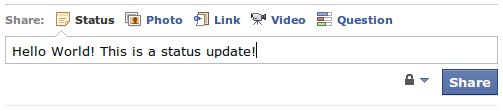
\includegraphics[width=12cm]{screens/control1.png}
                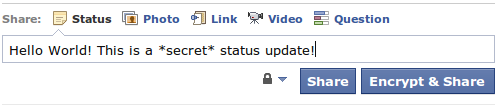
\includegraphics[width=12cm]{screens/control2.png}
            \caption{A control-field pair before (top) and after (bottom) parsing.}
            \label{scn:ctrl}
        \end{center}
    \end{figure}

Once a pair has been identified we generate an alternative encrypted submission control based on the existing control (see Figure \ref{scn:ctrl}). A handler is generated and associated with the input field. \footnote{For images this process is slightly different. A check box control is added and the handler to the normal control modified.}

The submission handler causes a friend selector window to appear (see Figure \ref{scn:fselector}) loaded with any friends whose public keys are stored on disk (see Section \ref{ssec:mankeys}). Elements within the control are populated with the user's names and profile pictures by performing queries through {\tt faceapi}.

    \begin{figure}[tbph]
        \begin{center}
                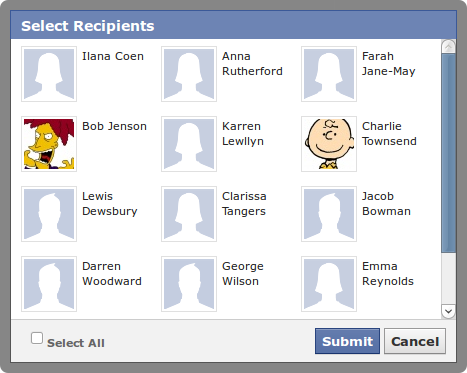
\includegraphics[width=10cm]{screens/fselector.png}
            \caption{Friend selector window.}
            \label{scn:fselector}
        \end{center}
    \end{figure}

On submission, the list of recipient's Facebook IDs and the input from the input field (either a text message or local image pathname) is gathered and processed by {\tt efb}. Sections \ref{sec:txt-sub} and \ref{sec:img-sub} describe this stage in detail. The result is a replacement input that can either be uploaded via {\tt faceapi} directly or alternatively uploaded via the original control-field pair.

\subsection{Identifying decryption targets}
\label{ssec:ident-targets}

Regular expressions are used to locate and filter possible decryption targets. For text these will be enclosed by special start and end sequences. Images can be identified by their filename as Graph API objects. In either case we take a best effort approach to filtering since a malicious user could easily create fake text tags and images are hard to filter out without first initiating decryption. The decryption process is designed to fail gracefully as early as possible if this turns out to be the case. \footnote{Currently, all ciphered images are $720 \times 720$ pixels allowing images to be filtered on their dimensions. The case for uploading variable sized images and its effect on filtering is discussed in Appendix \ref{app:imginc}.}

    
\subsection{Processing decryption targets}
\label{ssec:proc-targets}


Once a list of target Facebook IDs has been generated and filtered, it is processed. Each ID is checked to see if it has an entry in the cache. If not, an entry is created and a sequence of HTTP requests are triggered though {\tt efb}. For text this involves retrieving the note containing the ciphertext. For images this requires retrieving a full resolution copy of the image.\footnote{Most often images are displayed only as thumbnails. A full resolution copy of the ciphered image is obviously required to generate a plaintext thumbnail.} A handler is attached to the request so that on completion, the cache can be updated appropriately and parsing triggered. If an entry exists then several actions may be appropriate. If a valid plaintext exists exists in the cache this is used. The entry may also be marked as in progress in which case a loading message is substituted. If a previous attempt failed then the target can be ignored.

Parsing of a comment thread contained in a news feed is illustrated in figures \ref{scn:ctrl} and \ref{scn:ctrl2}. Note the CSS decoration demarcating an encrypted message.

    \begin{figure}[tbph]
        \begin{center}
                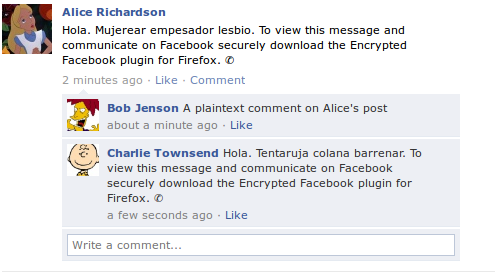
\includegraphics[width=12cm]{screens/content1.png}
                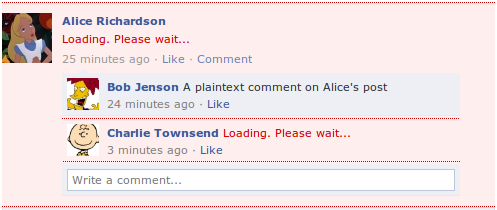
\includegraphics[width=12cm]{screens/content4.png}
            \caption{A news feed excerpt before (top) and after (bottom) parsing.}
            \label{scn:ctrl}
        \end{center}
    \end{figure}
    
    \begin{figure}[tbph]
        \begin{center}
        
                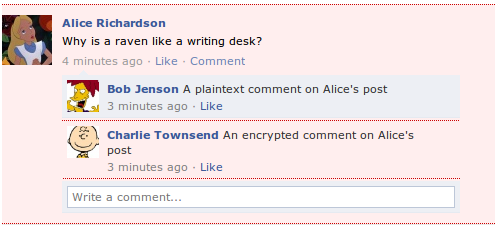
\includegraphics[width=12cm]{screens/content2.png}
                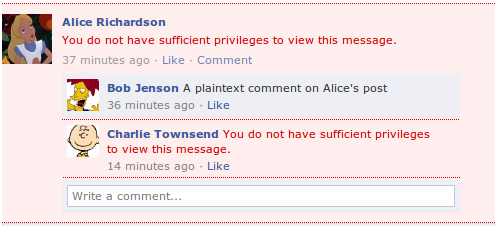
\includegraphics[width=12cm]{screens/content3.png}

            \caption{Two possible parsing outcomes given successful (top) or unsuccessful (bottom) decryption.}
            \label{scn:ctrl2}
        \end{center}
    \end{figure}
        

\FloatBarrier
\section{Key management}

A cryptographic identity\footnote{By which we mean a public-private key pair.} needs to be generated and uploaded before a user begins using the extension. Migrating identities is used to support use of the same identity from multiple devices. Public keys of other users also need to be downloaded and stored locally.


\subsection{Creating and migrating identities}

Creation and migration is performed through the browser toolbar (see Figure \ref{scn:pubkey}). On first install, only the {\tt [Create Identity]} button will be enabled. This action generates a local public-private key pair through the C++ module and uploads and appends the public key to the user's Bio attribute using {\tt faceapi} methods. Figure \ref{scn:bio} shows the key as it exists on a user's profile. The public key is encoded using Stego! (see Section \ref{ssec:submitnote}) and checks are made to prevent duplicate public keys existing online.

    \begin{figure}[tbph]
        \begin{center}
        
                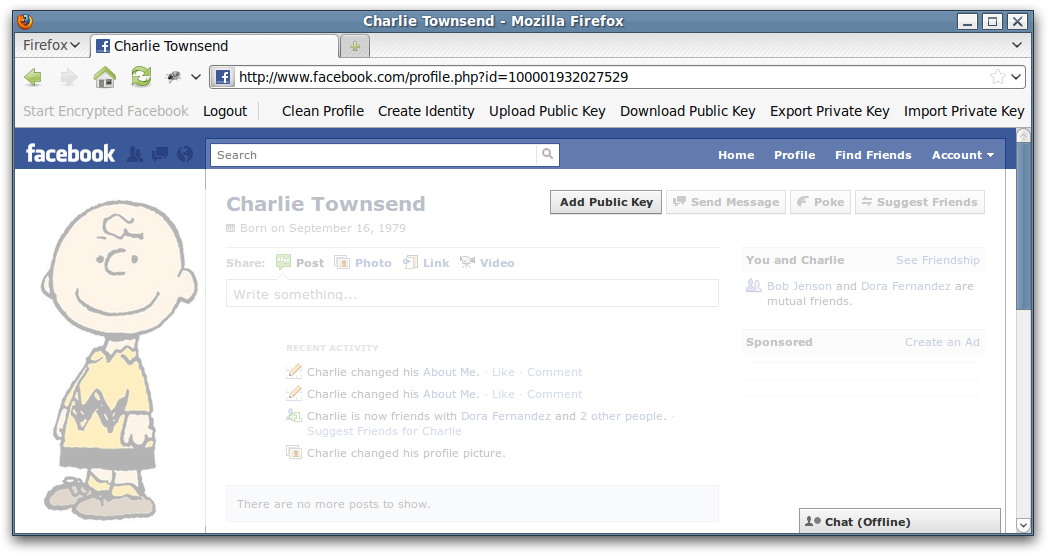
\includegraphics[width=12cm]{screens/pubkey.png}

            \caption{Key management controls located on the toolbar and within the profile itself.}
            \label{scn:pubkey}
        \end{center}
    \end{figure}

Migration of public keys can be performed in-band using the {\tt [Download Public Key]} toolbar control. The export and import controls for private keys require the user to securely transport the key file OOB.

    
\subsection{Managing public keys}
\label{ssec:mankeys}

Public keys are added and removed using a control on a user's profile page, inserted in a similar manner to submission controls. {\tt faceapi} is used to retrieve the Bio attribute and methods in {\tt efb} parse the result and write the public key out to a file using the Facebook ID as the filename. The local cache of public key files determines which users appear in the friend selector control.
    
        \begin{figure}[tbph]
        \begin{center}
        
                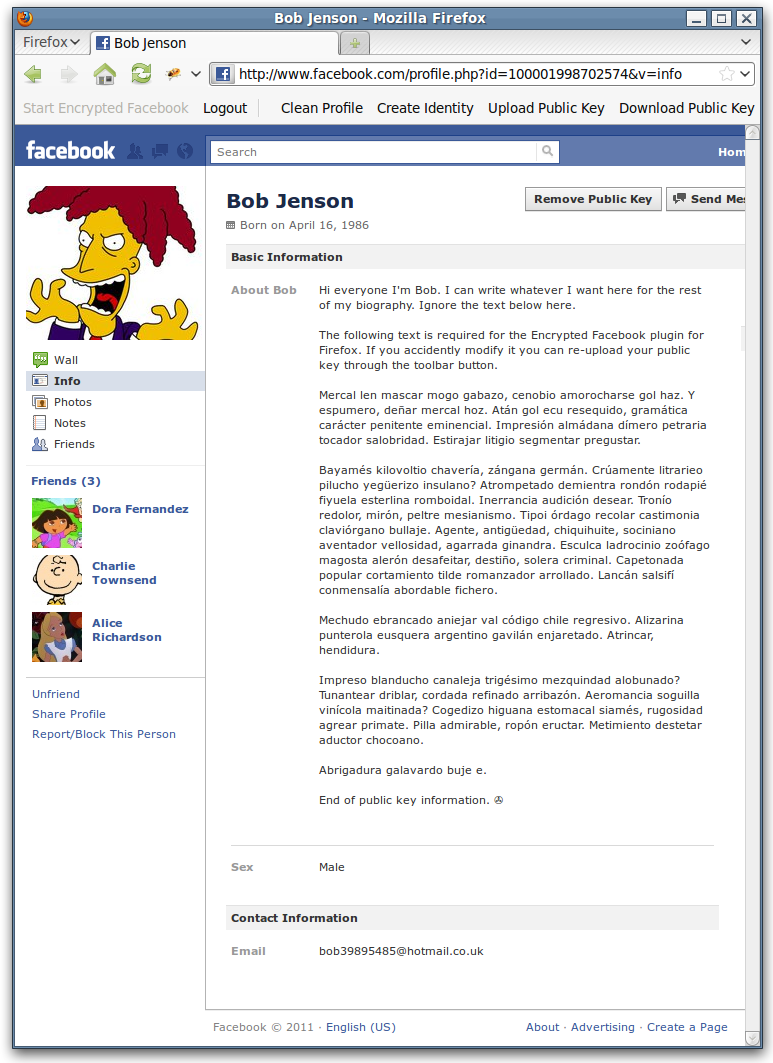
\includegraphics[width=12cm]{screens/bio.png}

            \caption{Public key encoded and stored in the user's biography section of their profile.}
            \label{scn:bio}
        \end{center}
    \end{figure}
    
Optionally, Encrypted Facebook will check if local public keys are up to date with online keys before submitting encrypted content. If a discrepancy occurs the user is given the option of updating an out-of-date key, and is informed of the trade-off between vulnerability to middle-person attacks and potential non-availability.

    
\FloatBarrier
\section{Text encoding}
\label{sec:txt-sub}

We consider the process by which a message, given a list of recipients, is transformed to an encoded tag which can then be used in place of the plaintext (Figure \ref{tikz:text}).

    \begin{figure}[tb]
        \begin{center}
                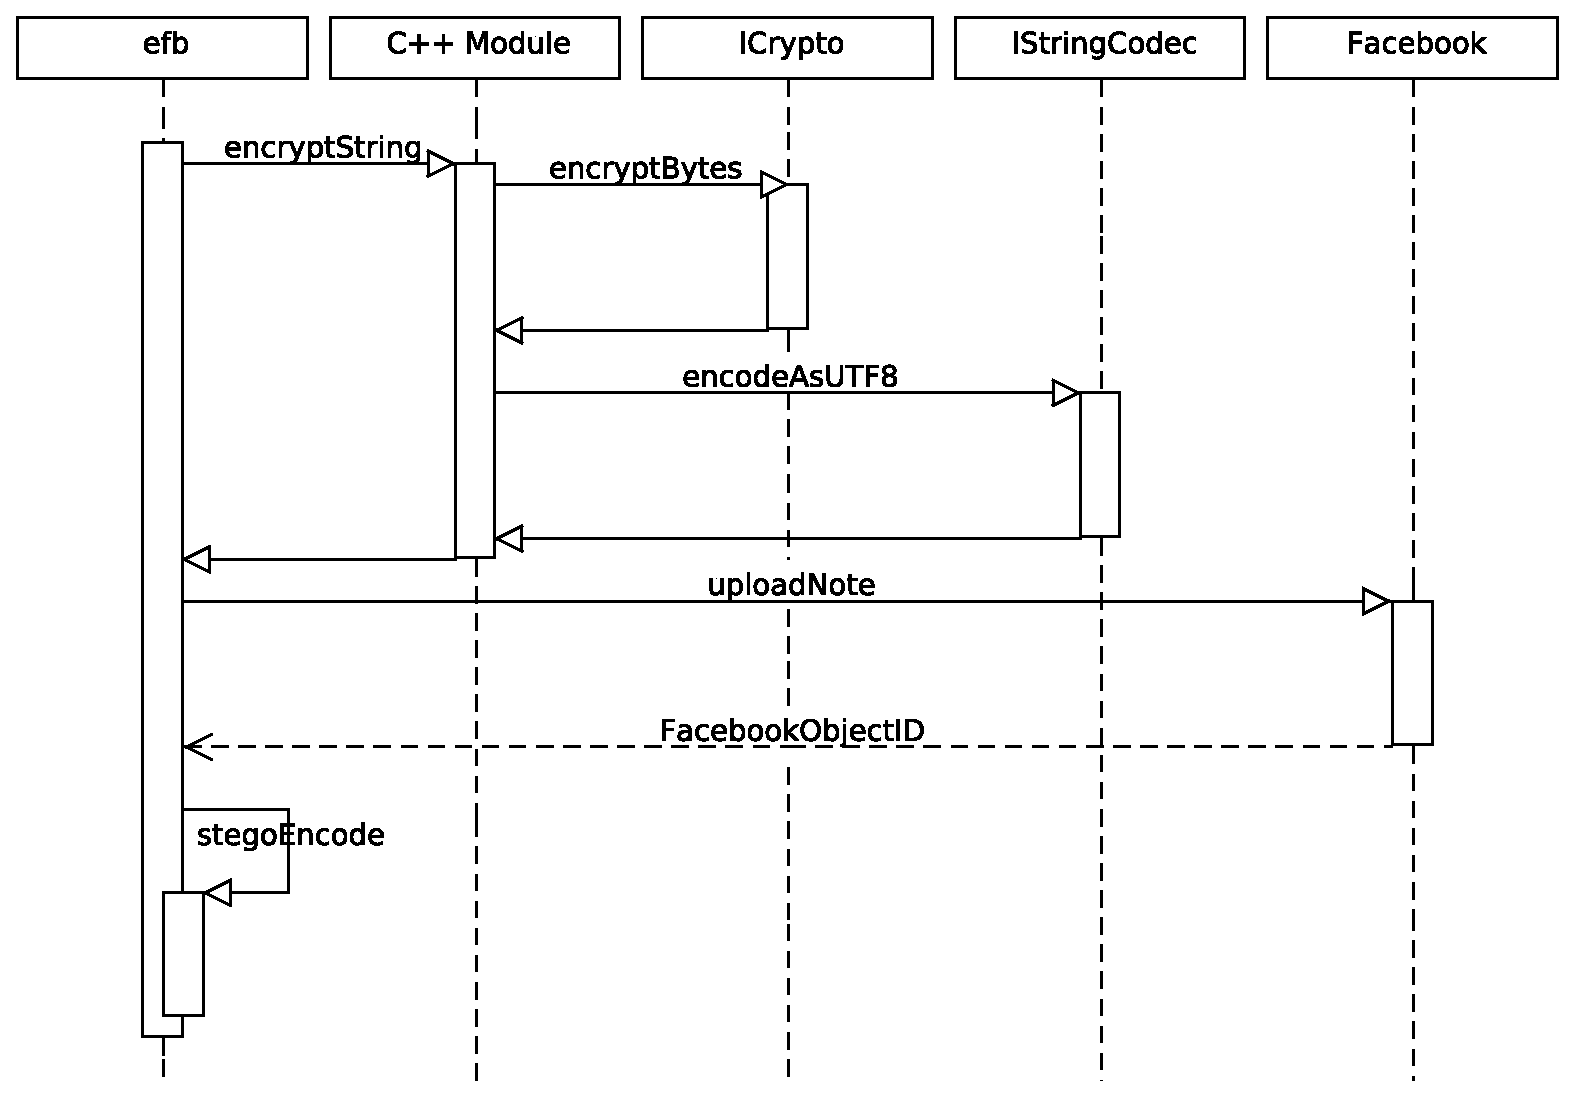
\includegraphics[width=12cm]{gfx/text-seq.eps}
            \caption{UML sequence diagram of the encoding process for submitting text.}
            \label{tikz:text}
        \end{center}
    \end{figure}

The message is passed to the C++ library, encrypted then encoded in a UTF-8 based format suitable for Facebook. The result is returned to the JavaScript module, submitted as a note to Facebook, and a tag generated from the resultant object ID using steganography.

Note that the tag does not contain the message itself, it points to the location on Facebook where the ciphertext can be obtained.

\subsection{Encryption}
\label{ssec:encrypt}

    \begin{figure}[tb]
        \begin{center}
                \includegraphics{gfx/crypto.1}
            \caption{UML class diagrams for the cryptography component.}
            \label{uml:crypto}
        \end{center}
    \end{figure}
    
Currently the only implementation for cryptographic functions is based on the Botan library using RSA and AES. The Botan library is encapsulated in a class with template parameters {\tt (N, M)} which determine the length (in bytes) of the AES session key and RSA public key, respectively. We designed this class in such a way that a class with certain key lengths\footnote{Obviously specified key lengths must be supported by Botan.} can be defined simply by specifying these parameters.
    
    \begin{table}[tb]
        \begin{center}
                \begin{tabular}{|+l|^l|}
                    \hline
                    \rowstyle{\bfseries}%
                    Description & Size (bytes) \\ \hline
                    \hline
                    Length tag & 2\\ \hline
                    Initialisation vector & 16 \\ \hline
                    Facebook ID & 8 \\ \hline
                    Session key & {\it <pub-key size>} \\ \hline
                    \multicolumn{2}{c}{$\vdots$} \\ \hline
                    Facebook ID & 8 \\ \hline
                    Session key & {\it <pub-key size>} \\ \hline                    
                \end{tabular}
            \caption{Structure of the encryption header.}
            \label{tab:crypto}
        \end{center}
    \end{table}
    
The input string is converted to a byte vector containing enough free space at the beginning for the encryption header\footnote{The size of the crypto header can be calculated in advance based on the recipient list, so that encryption can be performed in place.} along with a recipient list of Facebook IDs. The output is the ciphered message with the encryption header prepended.

Table \ref{tab:crypto} describes the format of the crypto header generated as part of the broadcast encryption scheme. Note that the public key size determines the cipher block size and therefore the storage requirements for the encrypted session key - regardless of the actual session key length itself.

The Botan SecureVector data structure is used to intermediately store all cryptographic keys, preventing key material being swapped to disk. A random IV and session key is generated for every message using Botan. After encryption, all seeds, key material and IVs are disposed of securely.


\FloatBarrier
\subsection{String coding}
\label{ssec:utf8}

The input to this stage is a byte vector of encrypted bytes. Each 16-bit (2 bytes) code is mapped on to a valid UTF-8 character - a variable length sequence of 1 to 5 bytes. Odd numbered input is padded and an otherwise unused character sequence prepended to indicate this. The mapping is based on the mapping from Unicode code points to UTF-8 chars, with two distinctions:

\begin{itemize}

    \item Each 16-bit input is shifted by an offset of 0xB0 before being mapped to a character. This avoids problem symbol characters which will be escaped by the Facebook sanitization process ('<' and '>' for example).
    
    \item Unicode code points {\tt U+D800} - {\tt U+DBFF} are surrogate pair characters and are illegal if used in isolation. Inputs which map to these characters (after being offset) are bit-shifted left by one place.
    
\end{itemize}


Note that this means some of the resulting characters are outside the BMP (Basic Multilingual Plane).

After adding a null terminal the final string can be returned to the JavaScript calling function.


\FloatBarrier
\subsection{Submission as a note}
\label{ssec:submitnote}

The final string is submitted as a note to Facebook via {\tt faceapi}, the relevant handlers being passed from {\tt efb}. An example result is shown in Figure \ref{scn:note}. On completion the 4-byte Facebook Graph API object ID is parsed from the {\tt XmlHttpRequest} response.  Start and end tags are added and the final text is ready to be used in place of the cleartext, as described in Section \ref{ssec:insert}.


    \begin{figure}[tbph]
        \begin{center}
                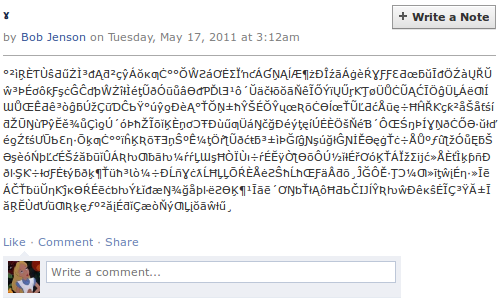
\includegraphics[width=10cm]{screens/note.png}
            \caption{A short example note as it exists on Facebook.}
            \label{scn:note}
        \end{center}
    \end{figure}

Two additional steps are also performed:

\begin{itemize}
    \item Firstly, a clean-up function is queued to run 1,2,4,8, and 16 seconds after submission. This will submit delete queries through {\tt faceapi} to remove unwanted notifications.
    
    \item Secondly, tags are encoded using the Stego! steganography library \footnote{Stego! outputs nonsensical sentences. We use a Spanish dictionary to partly conceal this fact.} rather than Base64 or the encoding scheme described in Section \ref{ssec:utf8}, to give a more pleasing aesthetic.
\end{itemize}

\FloatBarrier
\section{Image encoding}
\label{sec:img-sub}

We now describe the process by which an image, stored locally, is encrypted and encoded in a temporary image file ready to be uploaded.

The C++ library is passed the input and output file paths. Initially the image data is loaded from disk as a byte vector (leaving room for the encryption header) and encrypted exactly as described in Section \ref{ssec:encrypt}. Error correcting codes are then added. Finally, a conduit image object is created, written to, and saved to disk in a lossless format. We describe the last two stages in further detail.

    \begin{figure}[tb]
        \begin{center}
                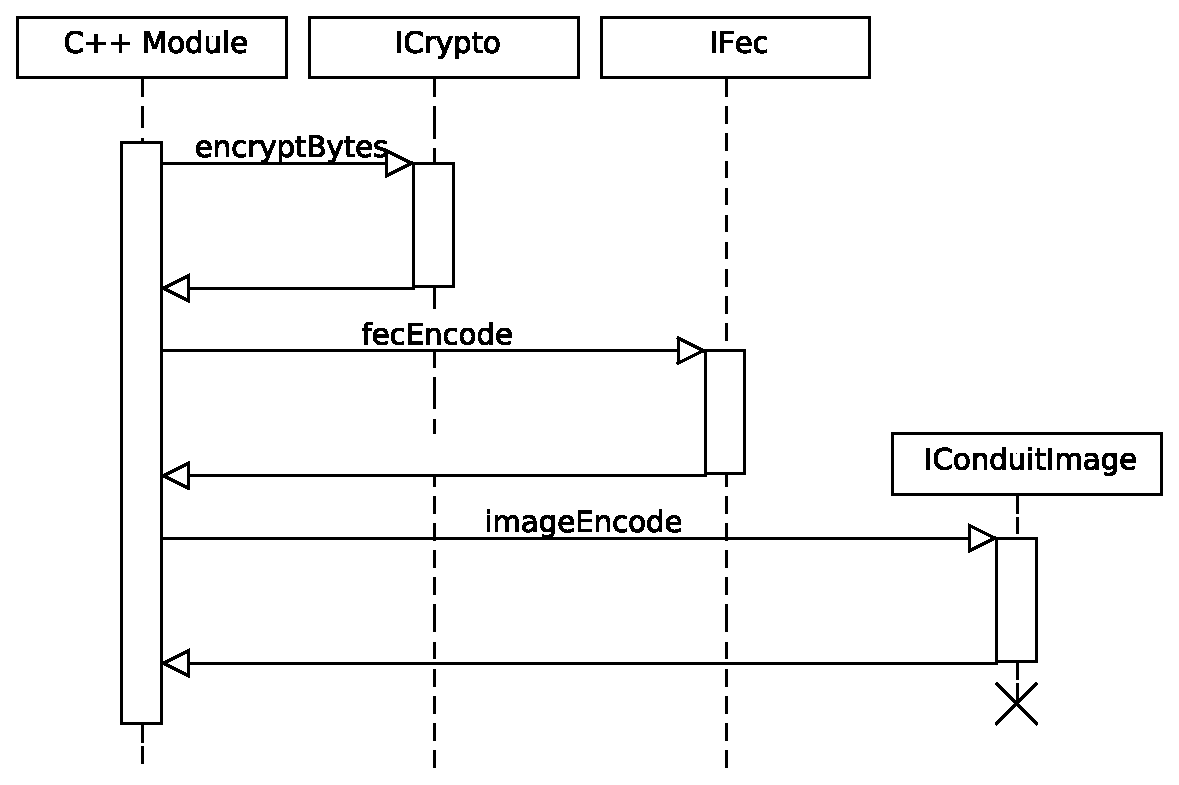
\includegraphics[width=12cm]{gfx/img-seq.eps}
            \caption{UML sequence diagram of the encoding process for submitting an image.}
            \label{eps:img}
        \end{center}
    \end{figure}


\FloatBarrier
\subsection{Forward error correction}

Currently the only FEC implementations are based on the Schifra library using Reed Solomon codes. The Shifra library is encapsulated in an abstract base class and two template specialisation subclasses implementing codes rates of (15,9) and (255,223) (see Figure \ref{uml:fec}).


    \begin{figure}[tb]
        \begin{center}
                \includegraphics{gfx/fec.1}
            \caption{UML class diagrams for the forward error correction library component.}
            \label{uml:fec}
        \end{center}
    \end{figure}

The FEC algorithms have a fixed block size. In order to avoid excess padding bytes or addition length tags, we use a scheme inspired by ciphertext stealing used in cryptography \cite{stealing}. The FEC codes are appended to the data bytes so that, provided there are enough blocks, any last partial block will be padded out automatically.

A length tag is also FEC encoded and appended so that padding bytes can later be removed.


\FloatBarrier
\subsection{Conduit image class hierarchy}

Images are encoded by generating an instance of IConduitImage through the abstract factory, writing data to it by calling the {\tt implantData} method, then saving out to disk. The {\tt CImg} class (from the CImg library) is used as a base class since it supports opening and saving various image formats, manipulating pixels and colour space transforms.

    \begin{figure}[tbp]
        \begin{center}
                \includegraphics{gfx/img.1}
            \caption{UML class diagrams for the conduit image implementation.}
            \label{uml:img-classes}
        \end{center}
    \end{figure}
    
{\tt implantData} begins by resizing the image to $720 \times 720$, greyscale. It then writes the data one byte at a time using the (protected) {\tt write} method defined in {\tt BufferedConduitImage}. The remainder of the image is padded with random bytes for aesthetic effect.

\FloatBarrier
\subsection{Read/write buffering}

All current conduit image implementations are derived from the abstract base class {\tt BufferedConduitImage} which supports reading and writing single bytes. Buffers are used to group read/write requests together to write to an abstract block --- the actual block implementation is left to the subclass. Each subclass defines a block as having certain dimensions and calls the parent constructor with {\tt block\_size}, the number of bytes one block can store. Examples are listing for three concrete subclasses in Table \ref{tab:blocks}.

The variables {\tt rhead} and {\tt whead} determine the current position of the read and write heads, or equivalently the number of bytes written or read since creation. Any subclass of {\tt BufferedConduitImage} must implement a method {\tt getBlockCoords} to map the position of the read/write heads to block coordinates within the image. Subclasses must also implement {\tt encodeInBlock} and {\tt decodeFromBlock} for writing {\tt block\_size} bytes to and from a block, given the block coordinates.

This class also contains Gray code translation functions, since they are used by all descendant classes and their definitions are too small to justify a class of their own. The Gray code length used varies depending on implementation (see Table \ref{tab:blocks}).

\begin{table}[tbph]
    \begin{center}
            
            \begin{tabular}{+l ^l ^l ^l}
                \rowstyle{\bfseries}%
                Class & \parbox[t][][t]{12ex}{\raggedright Dimensions (pixels)} & \parbox[t][][t]{12ex}{\raggedright Block size (bytes)} & \parbox[t][][t]{12ex}{\raggedright Grey codes (bits)} \\
                \midrule
                Haar WT & 8 $\times$ 8 & 3 & 6 \\
                3-bit Scaling & 3 $\times$ 2 & 3 & 3\\
                4-bit Scaling & 2 $\times$ 1 & 1 & 4
            \end{tabular}
            
        \caption{Comparison of blocks for each concrete subclass}
        \label{tab:blocks}
    \end{center}
\end{table}
    
\FloatBarrier
\subsection{Haar wavelet transform}

The {\tt HaarWTConduitImage} class uses blocks of 8x8 pixels (aligned with JPEG blocks) and a block size of 3-bytes. Two passes of the 2D Haar wavelet transform are performed on a single block. 6-bits are written to the high order bits of each of the four 8-bit approximation coefficients. The low order bits are masked off based on experimental results and suggestions in \cite{haar}. The inverse transform is then performed to output greyscale pixel values.

\begin{figure}
\begin{center}

    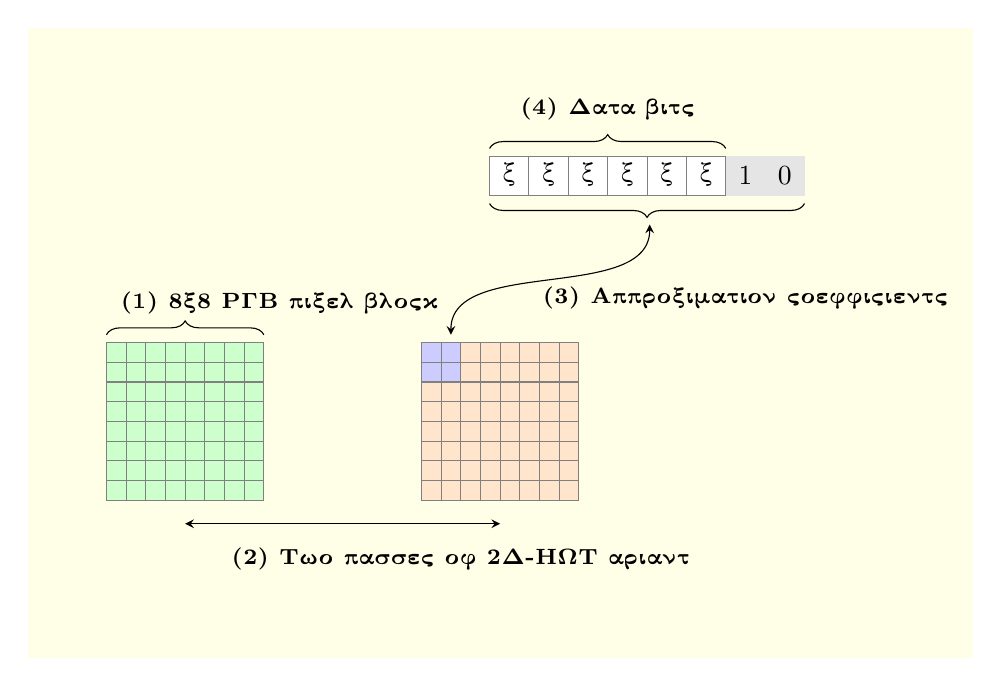
\begin{tikzpicture}[]


% bg bg

\fill[fill = yellow!10] (-2,-2) rectangle (10,6);

% bg
\fill[fill = green!20] (-1,0) rectangle (1,2);

\fill[fill = orange!20] (3-0.0001,0) rectangle (5,2);
\fill[fill = blue!20] (3-0.0001,1.5) rectangle (3.5,2);


% grids
\draw[step=0.25,color=black!50!white] (-1,0) grid (1,2);
\draw[step=0.25,color=black!50!white] (3-0.0001,0) grid (5,2);

% bits
\fill[xshift=110, yshift=110, fill = white] (3,0) (0,0) rectangle (4,0.5);
\draw[xshift=110, yshift=110, step=0.5,color=black!50!white, fill=white] (0,0) grid (4,0.5);



\draw[xshift=110, yshift=110] node at (0.25,0.25) {x};
\draw[xshift=110, yshift=110] node at (0.75,0.25) {x};
\draw[xshift=110, yshift=110] node at (1.25,0.25) {x};
\draw[xshift=110, yshift=110] node at (1.75,0.25) {x};
\draw[xshift=110, yshift=110] node at (2.25,0.25) {x};
\draw[xshift=110, yshift=110] node at (2.75,0.25) {x};

\draw [decorate,decoration={brace,amplitude=5pt}]
   (-1,2.1) -- (1,2.1);
\draw [decorate,decoration={brace,amplitude=5pt},xshift=110, yshift=110]
   (0,0.6) -- (3,0.6);
\draw [decorate,decoration={brace,amplitude=5pt},xshift=110, yshift=110]
   (4,-0.1) -- (0,-0.1);

\fill[xshift=110, yshift=110, fill = black!10!white] (3,0) rectangle (4,0.5);

\draw[xshift=110, yshift=110] node at (3.25,0.25) {1};
\draw[xshift=110, yshift=110] node at (3.75,0.25) {0};


% arrows

\draw[font={\footnotesize \bfseries}] node at (1.2,2.5) {(1) 8x8 RGB pixel block};


\draw[<->,>=stealth] (0,-0.3) -- (4,-0.3);
\draw[font={\footnotesize \bfseries}] node at (3.5,-0.75) {(2) Two passes of 2D-HWT variant};

\draw[<->,>=stealth] (3.375,2.1) .. controls (3.375,3.1) and (5.9,2.5) .. (5.9,3.5);
\draw[xshift=110, yshift=110, font={\footnotesize \bfseries}] node at (3.25,-1.3) {(3) Approximation coefficients};

\draw[xshift=110, yshift=110, font={\footnotesize \bfseries}] node at (1.5,1.1) {(4) Data bits};


\end{tikzpicture}
    
    \caption{Outline of the encoding process}
    \label{tikz:haar}
\end{center}
\end{figure}

The {\tt CImg} class does contain Haar transforms but these are not suitable. We require an integer lifting scheme (described in \cite{haar}) to ensure that the transform is reversible. In the 1-dimensional case, for a pair of approximation and difference coefficients $(c_a,c_d)$, we calculate the output value pair $(x,y)$: 

\begin{eqnarray}
    x = & c_a + \lfloor \frac{c_d+1}{2} \rfloor \nonumber \\ 
    y = & x - c_d
\end{eqnarray}

Iteration of the above over pairs in both vertical and horizontal axes can be used to perform the full 2D HWT and its inversion losslessly.

Changing the approximation coefficients can also lead to capping of values as they are mapped back to greyscale space, outside the 0-255 range. We therefore selectively discard high frequency information (during the inverse transform) from the difference coefficient $c_d$ whenever capping occurs - leaving the approximation coefficients intact and the output within range.



\FloatBarrier
\subsection{N-bit scaling}

The abstract base class {\tt ScaledConduitImage} contains functions to code n-bits of data to and from a single pixel using the n-bit scaling method. The value of n is set on instantiation.

Two subclasses are specified for $n=3$ and $n=4$. For $n=3$ we use 3x2 blocks of pixels with a block size of 3-bytes. For $n=4$ we use blocks of 2 pixels with a block size of 1-byte.

The scaling process works so that the intervals for each data point are of equal width, except for the intervals at either end which are $\frac{1}{2}$ length. This is because extreme values (0 or 255) can only be either decreased or increased due to compression artefacts, not both. An input pixel value of 255 might result in 254 or 253 after compression, but never 0 or 1.

    
\begin{figure}[htp]
  \begin{center}
    \subfigure[{\it HWT method}]
        {\label{fig:edge-a}
\includegraphics[width=4cm]{screens/haar.jpg}}
    \subfigure[{\it 3-bit scaling method}]
        {\label{fig:edge-b}
\includegraphics[width=4cm]{screens/scaled3.jpg}}
    \subfigure[{\it 4-bit scaling method}]
        {\label{fig:edge-b}
\includegraphics[width=4cm]{screens/scaled4.jpg}}
  \end{center}
  \caption{Final output of the image coding process.}
  \label{scn:images}
\end{figure}
    

\FloatBarrier
\section{Testing}

Many modules or processes could be unit tested individually before being aggregated and integration testing performed. Note that this section does not describe the chronology of development. In accordance with an agile developmental approach the focus was on delivering a minimally functioning prototype as early in the development life-cycle as possible, combining aspects of all the components listed below. Iterative improvement and development was then performed until a fully functioning system emerged.


\subsection{Page interception module}

The {\tt pagecept} parsing module was present in early prototypes, with placeholder messages and images used to demarcate decrypted items and skeleton handlers attached to UI controls. Testing principally involved manual inspection of the DOM using FireBug to ensure parsing had occurred correctly. Test scripts derived from boundary-value analysis (details in Appendix \ref{app:bv}) were also run using FireBug and FireUnit to test that DOM insertions were being sanitised correctly. The cognitive walkthrough method was also performed periodically to identify usability issues with UI controls, which could then be fixed.

Initially a small subset of decryption target types and control-input pairs were supported. As development progressed each successive prototype added wider support for more specific cases. Testing was tightly integrated with and performed throughout development, in line with agile testing methodology.


\subsection{Image coding}

Development of image coding algorithms, particularly the HWT method, was highly susceptible to conceptual bugs. Abnormal error rates were, in some cases, the only indicator that a bug was present, and had to be carefully monitored during development. Testing involved simulating compression using the IJG {\tt libjpeg} library --- initially for single $8 \times 8$ blocks then later for entire images. Extraneous library methods were coded for calculating the Hamming distance, edit distance and other metrics between byte sequences and/or files. A standalone test instance of the C++ library was used since starting and stopping the browser was considerably time consuming.


\subsection{Other modules}

The UTF-8 codec was also tested using boundary-value analysis (details in Appendix \ref{app:bv}). 

Layers of encoding for both text and images were added to successive prototypes. Encoding layers could then be turned on and off during testing with command line switches to isolate bugs to specific library components.


\subsection{Integration testing}

Eventually simulation of the JPEG compression process was replaced by automated uploading and downloading of images to and from Facebook.

Particular care was taken to ensure text sanitisation was tested end-to-end, including submission and retrieval to/from Facebook, since the complexity of the UTF-8 coding scheme and the custom built decoder introduced the possibility of bypassing sanitisation \cite{utf8}.

\cleardoublepage%*****************************************
\chapter{Evaluation}\label{ch:evaluation}
%*****************************************
\label{eval}

In this chapter we investigate how the choice of image coding implementation affects bit error rates and capacity, and how the recipient group size affects codec performance. We also look at the effect of clearing the extension cache on page loading times and present some outcomes of the usability inspection.

Test data was generated on a laptop running Linux Mint 10.0 using a 1.46 Ghz Intel Pentium dual core CPU with 1 GiB of RAM. A 10 Mbpbs broadband connection was used to connect to the internet, with measured download/upload rates of around 8 Mbps and 2 Mbps respectively. For comparison, Firefox 4.0's minimum requirements include a single core 1.4 Ghz CPU with 512 MB of RAM \cite{firefox-req}. The average broadband speed in the UK is around 10 Mbps \cite{bband-stats}. 

\section{Image coding method}
\label{sec:imgcod}

We investigate how the concrete {\tt IConduitImage} implementation affects bit error rates and theoretical image capacity. The capacity puts a maximum limit on the number of possible recipients an image can be shared with, and also limits the size of the image. In addition, error rates determine which error correction schemes are most suitable and what the final output error rate will be after application of a given scheme.

We test the hypothesis that the HWT, 3-bit scaling and 4-bit scaling methods provide both greater capacity and lower error rates than the naive methods described in Section \ref{ssec:naive} after undergoing Facebook's image upload process.

\subsection{Method}

In this instance, local simulation with {\tt libjpeg} was used since uploading to Facebook on this scale would be considerably time consuming and would possibly warrant account deletion due to violation of Facebook's terms. We compress over the quality factor interval 80-90 --- though it is most likely that Facebook uses IJG quality factor 85, this is only an estimate. This also means our results are somewhat robust to minor changes in Facebook's compression process.

We model the compression/decompression process as a binary symmetric channel and calculate the channel capacity for arbitrarily small error probability, using an empirically measured bit error rate as an estimate for the bit error probability.

Random input bytes are written to a $720 \times 720$ conduit image instance until full. The image is then saved as a JPEG at a given quality factor, reloaded and the data extracted. We record the Hamming distance between the input and output data. This process is repeated until the cumulative amount of data processed exceeds 1 GiB.

\begin{table}[tbph]
  \begin{center}
        \begin{tabular}{l l l l l}
        \textbf{Method} &\textbf{Bits per} &\textbf{Test set size} & \textbf{Test set size} &\textbf{Possible unique} \\ 
            &\textbf{block} &\textbf{(images)} &\textbf{(blocks)} &\textbf{blocks} \\ [0.1ex] \hline \\ [-1.5ex]
        Scaled3	&192	&5,523	&44,736,300	& $6.28 \times 10^{57}$ \\
        Scaled4	&256	&4,142	&33,550,200	& $1.16 \times 10^{77}$ \\
        Haar	&24	&44,186	&357,906,600	& $1.68 \times 10^{7}$ \\
        \end{tabular}
        \caption{Tabulated details of the testing process.}
        \label{tab:img-test}
    \end{center}
\end{table}

Table \ref{tab:img-test} summarises the number of useful bits each method can store in a single 64 x 8 bit greyscale JPEG luminance block along with the effective sample size and population size. Due to the number of samples the standard error is negligible, even before applying finite population correction where appropriate \footnote{In particular, for the Haar wavelet transform method the number of JPEG blocks encoded exceeds the number of unique data points that can be encoded in a single block.}. 

\subsection{Theoretical capacity calculation}

The per-image theoretical capacity $C$ is a function of the number of bits available per image $A$\footnote{Determined by the implementation.} and the bit error probability $p_e$:

\begin{equation}
    C = A \cdot (1 + H(p_e))
\end{equation}

where $H(x)$ is the binary entropy function. This provides the capacity in units of information per symbol, or in our case KiB per image.

\subsection{Results}

Both n-bit scaling methods showed marked improvements in error rates and capacity (see Figure \ref{graph:ber} and Figure \ref{graph:capacity}) in comparison to naive approaches.

The HWT method, however, had the lowest capacity of all methods tested. We attribute this mainly to the fact that two passes of the HWT were required to successfully reduce error rates, and that, due to the nature of the method, each pass reduces capacity by a factor of 4. The final error rates obtained do at least support the claim made in \cite{haar} that such an encoding scheme is reasonably immune to JPEG compression.


\begin{figure}[tbph]
  \begin{center}
\begin{tikzpicture}
    \begin{axis}[grid=major,xlabel=JPEG Quality Factor,ylabel=BER (\%), xmin=80, xmax=90,
    height=8cm,width=10cm,legend style={legend pos=outer north east}]
    \addplot
        table[x=QF,y=Sc3] {gfx/error_rate.data};
    \addplot
        table[x=QF,y=Sc4] {gfx/error_rate.data};
    \addplot[mark=diamond*, color=green]
        table[x=QF,y=Haar] {gfx/error_rate.data};
        
    \addplot[mark=triangle*, color=purple]
        table[x=QF,y=rgb] {gfx/error_rate0.data};
    \addplot[mark=diamond*, color=orange]
        table[x=QF,y=dct] {gfx/error_rate0.data};
    
    \legend{Scaled3,Scaled4,Haar,Pixels,DCT}
    \end{axis}
\end{tikzpicture}
    \caption{Bit error rate for varying quality factors.}
    \label{graph:ber}
  \end{center}
\end{figure}

\begin{figure}[tbph]
  \begin{center}
\begin{tikzpicture}

    \begin{axis}[grid=major,xlabel=JPEG Quality Factor,ylabel=Capacity (KiB/image), xmin=80, xmax=90,
    height=8cm,width=10cm,legend style={legend pos=outer north east }]
    \addplot
        table[x=QF,y=Sc3] {gfx/encoding_time.data};
    \addplot
        table[x=QF,y=Sc4] {gfx/encoding_time.data};
    \addplot[mark=|, color=green]
        table[x=QF,y=Haar] {gfx/encoding_time.data};
        
    \addplot[mark=triangle*, color=purple]
        table[x=QF,y=rgb2] {gfx/error_rate0.data};
    \addplot[mark=diamond*, color=orange]
        table[x=QF,y=dct2] {gfx/error_rate0.data};
        
    \legend{Scaled3,Scaled4,Haar,Pixels,DCT}
    \end{axis}
\end{tikzpicture}
    \caption{Per-image channel capacity (measured in KiB/image) for varying quality factors.}
    \label{graph:capacity}
  \end{center}
\end{figure}

\subsection{Implications}

We can compare the capacity limit obtained in the previous section to the actual capacity achieved when an error correction scheme is applied (see Table \ref{tab:fec}).

We can also use the estimation of bit error probability to calculate the probability of decoder output error. Given the bit error probability $p$ we can obtain the symbol error probability $p_s$:

\begin{equation}
    p_s = 1 - (1-p)^m
\end{equation}

where $m$ is the number of bits per symbol. In general, for a Reed Solomon code with symbol error probability $p_s$ the decoded symbol error probability $p_s'$ is given by:

\begin{equation}
    p_s' = \frac{1}{2^m -1} \sum^{2^m - 1}_{i = t+1} i {{2^m - 1}\choose{i}} {p_s}^i (1-{p_s})^{2^m - 1 - i}
\end{equation}

where $t$ is the maximum number symbol errors we can correct \cite{rsfec-decode}. The resulting decoder output error rates, along with achievable capacity, are shown in Table \ref{tab:fec} for JPEG quality factor 85.

\begin{table}[tbph]
  \begin{center}
        \begin{tabular}{l l l l l l}
            
            \textbf{Method} & \textbf{FEC} & \textbf{$p$} & \textbf{$p_s$} & \textbf{$p_s'$} & \textbf{Capacity} \\  & &  &  &  & \textbf{(KiB)} \\[0.1ex] \hline \\ [-1.5ex]

            Haar & (15,9) & $4.20 \times 10^{-3}$ & $1.67 \times 10^{-2}$ & $2.47 \times 10^{-5}$ & 14.2 \\
            Haar &  (255,223) & $4.20 \times 10^{-3}$ & $3.31 \times 10^{-2}$ & $3.73 \times 10^{-4}$ & 20.8 \\
            Scaled3 & (15,9) & $8.30 \times 10^{-4}$ & $3.32 \times 10^{-3}$ & $4.28 \times 10^{-8}
$ & 113.9 \\
            \rowcolor{green!20!white} Scaled3 & (255,223) & $8.30 \times 10^{-4}$ & $6.62 \times 10^{-3}$ & $1.81 \times 10^{-13}
$ & 166.0 \\
            Scaled4 & (15,9) & $4.49 \times 10^{-2}$ & $1.68 \times 10^{-1}$ & $7.14 \times 10^{-1}$ & 151.9 \\
            Scaled4 & (255,223) & $4.49 \times 10^{-2}$ & $3.08 \times 10^{-1}$ & $3.08
 \times 10^{-1}$ & 221.4 \\
            
        \end{tabular}
        \caption{Bit error probability, symbol error probability and output symbol error probability for each possible combination.}
        \label{tab:fec}
    \end{center}
\end{table}

The 4-bit scaling class results in error rates too large to be corrected with the Reed Solomon codes used here, indicating that a different FEC scheme would be appropriate.

Using the 3-bit scaling class along with (255,223) FEC codes (highlighted in green) we would expect less than one bit error in a terabyte of encoded data. For comparison, this approaches hard disk drive read error rates \footnote{Stated by at least one hard drive vendor to be 1 uncorrectable read error in $10^{14}$ bits, or 10 terabytes \cite{hdd-errors}.}. The capacity (approximately 165 KiB) is also within 10\% of the Shannon limit for 3-bit scaling. We focus on this combination for the remainder of the evaluation.



\FloatBarrier
\section{Recipient group size}
\label{sec:recsize}

We investigate how recipient group size affects encoding and decoding performance. Large or highly variable decoding times would have an adverse effect on usability, in particular since decoding is triggered automatically whilst browsing. Potentially, practical recipient group sizes might be limited due to performance issues.

\begin{figure}[tbph]
    \begin{center}
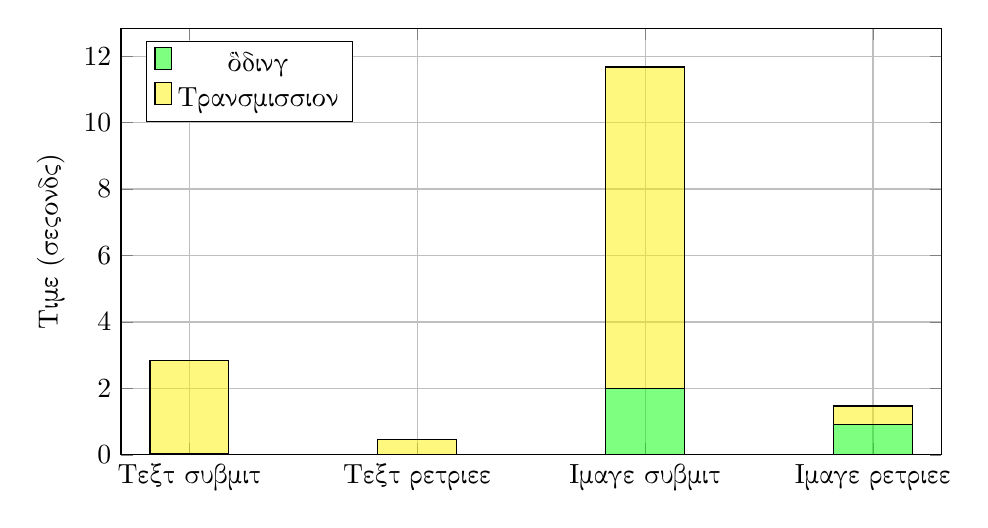
\begin{tikzpicture}
\begin{axis}[grid=major,ybar stacked, 
    symbolic x coords={Text submit,Text retrieve, Image submit, Image retrieve},
    xtick=data,ylabel=Time (seconds), width=12cm, height=7cm,
    legend style={legend pos=north west, area legend},
    bar width=1cm, ymin=0]

    \addplot[fill=green, fill opacity=0.5] coordinates
        {(Text submit,0.0444) (Text retrieve,0.0172) (Image submit,2.0074) (Image retrieve,0.9044)};
    \addplot[fill=yellow, fill opacity=0.5] coordinates
        {(Text submit,2.8013) (Text retrieve,0.4446) (Image submit,9.6655) (Image retrieve,0.5662)};
    \legend{Coding,Transmission}

\end{axis}
\end{tikzpicture}
    \caption{Average timing results for a 10,000 character note and an (approximately) 50 KiB image.}
    \label{graph:txt-sync}
  \end{center}
\end{figure}

Preliminary tests (see Figure \ref{graph:txt-sync}) show that time spent encoding and decoding text is too short to be an issue in any case. Therefore, we test the hypothesis that recipient group size has an  effect on image codec performance and measure the extent of this effect.



\subsection{Method}

A 50 KiB random test image was encrypted using 248-bit AES and 2048-bit RSA, encoded into a lossless image format.\footnote{Using 3-bit scaling and (255,223) Reed Solomon codes.} For each test the number of recipients was increased, from 1 up to a maximum of 400. Recipients were duplicates and selected at random from a pool of 15. The image was then compressed using {\tt libjpeg} and the data deciphered. Encode and decode times were recorded and included writing to and from disk but not JPEG compression. Checks were made to ensure that no decode errors occurred.

\subsection{Results}

\begin{figure}[tbph]
    \begin{center}
    
\begin{tikzpicture}
\begin{axis}[grid=major,
    xlabel=Recipient group size, ylabel=Encoding Time (seconds), height=10cm,width=10cm,
    ymin=0, xmin=0, xmax=400, legend style={legend pos=south west, empty legend}]
    
    \addplot[only marks, mark=x] table[x=r,y=t]
        {gfx/submit.data};
    \addplot[no marks, color=red] table[x=r,y={create col/linear regression={y=t}}]
        {gfx/submit.data};
    \addlegendentry{Slope = $\pgfmathprintnumber{\pgfplotstableregressiona}$};
    \addlegendentry{R = $\pgfmathprintnumber{0.726}$}

\end{axis}
\end{tikzpicture}

\begin{tikzpicture}
\begin{axis}[grid=major,
    xlabel=Recipient group size, ylabel=Decoding Time (seconds), height=10cm,width=10cm,
    ymin=0, xmin=0, xmax=400, legend style={legend pos=south west, empty legend}]
    
    \addplot[only marks,mark=x] table[x=r,y=t]
        {gfx/retrieve.data};
    \addplot[no marks, color=red] table[x=r,y={create col/linear regression={y=t}}]
        {gfx/retrieve.data};
    \addlegendentry{Slope = $\pgfmathprintnumber{\pgfplotstableregressiona}$};
    \addlegendentry{R = $\pgfmathprintnumber{0.615}$}

\end{axis}
\end{tikzpicture}

    \caption{Encoding (top) and decoding (bottom) times as recipient numbers increase.}
    \label{graph:subrep}
  \end{center}
\end{figure}

The results in Figure \ref{graph:subrep} show a significant linear correlation between group size and codec performance ($p < 0.001$). For both decoding and encoding, a group size of 400 incurs an average time overhead of less than 8\% compared to a single recipient.


\subsection{Implications}

Given a group size of $n$ and public key size $p$ the transmission overhead, in bytes, is given by:

\begin{equation}
    (n \times (4 + p)) + 16
\end{equation}

The implementation used for testing has a capacity of 165 KiB, which must include both the transmission overhead and the image itself. Thus group sizes larger than 400 are already approaching the capacity limit. Even given increased capacity, our results show that performance issues are unlikely to be the limiting factor to recipient group sizes.


\section{Plaintext caching}
\label{sec:ptextc}

Due to the nature of the parsing process (see Section \ref{ssec:proc-targets}) a cache of plaintext content accumulates on the user's machine. This cache can be cleared to decrease storage utilisation or for security purposes\footnote{Specific attacks involving the cache are not included in our initial threat model since they involve a malfeasor having access to the user's machine, a scenario which is considered a threat in itself.}, though this is likely to have a negative effect on response times and therefore on usability.

We test the hypothesis that clearing the plaintext cache increases page load times and estimate the worst case increase.


\subsection{Method}

Sample news feeds were generated with 15 encrypted status update entries, as this is the number of news feed entries Facebook first loads \footnote{More are loaded dynamically when the user scrolls to the bottom of the page.}. Status update messages were random ASCII text 420 characters in length, the maximum permitted. The pages were loaded repeatedly 400 times, ensuring that both the browser cache and extension cache were cleaned after each load.

The entire process was then repeated for a news feed containing 15 image objects, once again random images of size 50 KiB, instead of status messages. A second set of tests were performed without cleaning the extension cache (which was preloaded with the page's content).

The start time of each test was logged, along with the subsequent load times of the encrypted objects. 

    \begin{figure}[tbph]
        \begin{center}
                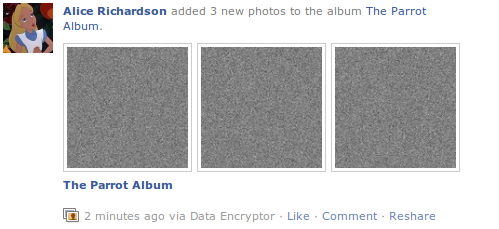
\includegraphics[width=10cm]{screens/parrots1.png}
                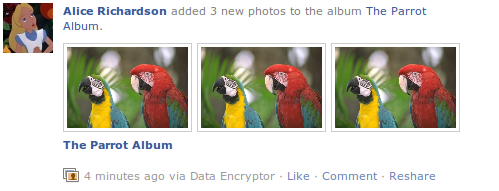
\includegraphics[width=10cm]{screens/parrots2.png}
            \caption{News feed excerpt containing encrypted image thumbnails, before (top) and after (bottom) parsing.}
            \label{scn:parrots}
        \end{center}
    \end{figure}


\subsection{Results}

The effect of plaintext caching on the overall page loading times can be seen in Figure \ref{graph:hist}. On average, load times for the entire page and all encrypted items were increased roughly by a factor of 2 for the feed containing just text and by a factor of 5 for the feed containing images. 

\begin{figure}[tbph]
    \begin{center}
\begin{tikzpicture}
\begin{axis}[xlabel=Time (seconds), ylabel=Frequency,
grid=major,const plot, ymin=0, enlargelimits=false,
width=12cm, height=5cm, legend style={area legend}]

    \addplot[fill=blue, fill opacity=0.5] table[x=t,y=Text] {gfx/async_text_hist.data};
    
    \addplot[fill=red, fill opacity=0.5] table[x=t,y=Text_c] {gfx/async_text_hist.data};
    
    \addplot+[sharp plot,blue, mark=no marker] coordinates
        {(6.403,0) (6.403,56)};
        
    \addplot+[sharp plot,red, mark=no marker] coordinates
        {(3.463,0) (3.463,56)};
    
    \legend{Cache off,Cache on}
\end{axis}
\end{tikzpicture}

\begin{tikzpicture}
\begin{axis}[xlabel=Time (seconds), ylabel=Frequency,
grid=major,const plot, ymin=0, enlargelimits=false,
width=12cm, height=5cm, legend style={area legend}]
    
    \addplot[fill=blue, fill opacity=0.5] table[x=t,y=Images] {gfx/async_image_hist.data};
    
    \addplot[fill=red, fill opacity=0.5] table[x=t,y=Images_c] {gfx/async_image_hist.data};
    
    \addplot+[sharp plot,blue, mark=no marker] coordinates
        {(19.169,0) (19.169,130)};

    \addplot+[sharp plot,red, mark=no marker] coordinates
        {(4.067,0) (4.067,130)};
    
    \legend{Cache off,Cache on}
    
\end{axis}
\end{tikzpicture}
    \caption{Histogram of 400 page loading times for news feeds containing 15 encrypted messages (top) and 15 encrypted images (bottom).}
    \label{graph:hist}
  \end{center}
\end{figure}

After the first item has loaded we can also look at the subsequent waiting time between loads. The most dramatic increase is for images, as seen in Table \ref{tab:async}.

\begin{table}[tbph]
  \begin{center}
        \begin{tabular}{+l ^l ^l ^l ^l}
            \rowstyle{\bfseries}%
            Element & \multicolumn{2}{^l}{Text (ms)} & \multicolumn{2}{^l}{Image (ms)}  \\
            \midrule 
            2 &	    30.6 &	2.6 &	782.3 &	6.5 \\
            3 &	    53.9 &	2.3 &	752.0 &	6.5 \\
            4 &	    29.0 &	2.3 &	761.6 &	6.4 \\
            5 &	    48.3 &	2.3 &	757.8 &	6.3 \\
            6 &	    48.9 &	2.3 &	781.0 &	6.4 \\
            7 &	    62.4 &	2.3 &	755.8 &	6.4 \\
            8 &	    113.4 &	2.4 &	769.8 &	6.5 \\
            9 &	    162.4 &	2.3 &	763.6 &	6.5 \\
            10 &    60.0 &	2.2 &	752.5 &	6.4 \\
            11 &    52.8 &	2.3 &	623.2 &	6.5 \\
            12 &    60.0 &	2.3 &	928.3 &	6.5 \\
            13 &    62.3 &	2.3 &	698.8 &	6.4 \\
            14 &    57.1 &	2.4 &	715.2 &	6.4 \\
            15 &    116.5 &	2.4 &	376.0 &	6.4
        \end{tabular}
        \caption{Page load times with (left column) and without (right column) cache cleansing beforehand.}
        \label{tab:async}
    \end{center}
\end{table}


\subsection{Implications}

Currently the plaintext cache is wiped on initialisation and destruction. Based on our results, most users would likely benefit from lengthening the cache expiration period, unless the extension was used mainly for text communications rather than image sharing. A full study of how the cache increases in size over time would required to make this judgement however; this was unfortunately not possible in the limited evaluation timeframe.





\FloatBarrier
\section{Usability inspection}
\label{sec:cw}

We present the final outcome of the usability inspection that was used as part of the development process. For the sake of concision we evaluate only the submission process for comments and images, as these contain the longest sequences of actions required of a user. The full set of tests is included in Appendix \ref{app:cw}.

We test the hypothesis that a typical Facebook user can successfully share an encrypted image, and that a similar user can successfully submit to that image an encrypted comment.


\subsection{Method}

We use the cognitive walkthrough (as described by Wharton et al \cite{cogwalk}) to evaluate the success of the user interface. This section consists of two of the final success stories and a defence of their validity. They refer to claims demonstrated by other walkthroughs which can be found Appendix \ref{app:cw}.

We only consider one class of user - a typical Facebook user who is therefore familiar with the Facebook user interface. It is therefore assumed that actions such as "navigate to a given friend's profile" can be performed without additional aid. It is also assumed that the user will follow their usual actions when trying to perform an encrypted operation - when trying to upload an encrypted image they will, for example, simply follow the normal procedure for uploading an image rather than searching for some hidden option. Finally, we make the assumption that the extension has been installed and enabled and that the toolbar has not been hidden.


\subsection{Uploading an encrypted image}
A user wishing to send an encrypted image to 405 friends who also have the extension, does so.

\begin{desc}

    \item[Action Sequence] \hfill
    \begin{enumerate}
        \item Add any public keys required.
        \item Navigate to the image upload page for the required album (see Figure \ref{scn:pic-up}).
        \item Select the image to encrypted.
        \item Check the {\tt [Encrypt]} check box.
        \item Click the {\tt [Submit]} button.
        \item Use the friend selector to select recipients and submit.
    \end{enumerate}
    
    \item[Defence of Credibility] \hfill
        \begin{itemize}
            
            \item The user knows he must add public keys of recipients beforehand and how to do so. If the user has no public keys Appendix \ref{app:cw:addkey} demonstrates that he will be able to add one of his intended recipients. Since the process is reasonably simple - simply navigate to their page and click a clearly marked button, we assume that any user who has performed it once can do so again if they wish, without further instruction. The link between adding public keys and being able to choose those friends as recipients should be fairly obvious; when the first key is added and encryption attempted again that same friend will appear as the only possible recipient.
            
            \item Facebook user will be familiar with the process of uploading an image. We assume a user trying to upload an encrypted image will be likely to try the method they are already familiar with.
            
            \item User knows things are OK since he sees the encryption check box option on arriving at the upload page. Check box leaves little room for confusion over whether an upload will or won't be encrypted.
            
            \item User knows to select an image to upload since the process is identical to uploading plaintext images.
            
            \item User knows to select {\tt [Encrypt]} check box since uploading an encrypted image is the original task.
            
            \item User knows things are OK since the recipient selector pops up.
            
            \item User knows how to use the recipient selector (see Appendix \ref{app:cw:sel}).
            
            \item User knows things are OK as Facebook handles the upload process from here as per normal, notifying user when the upload is complete.
            
        \end{itemize}
    
\end{desc}


    \begin{figure}[tbph]
        \begin{center}
        
                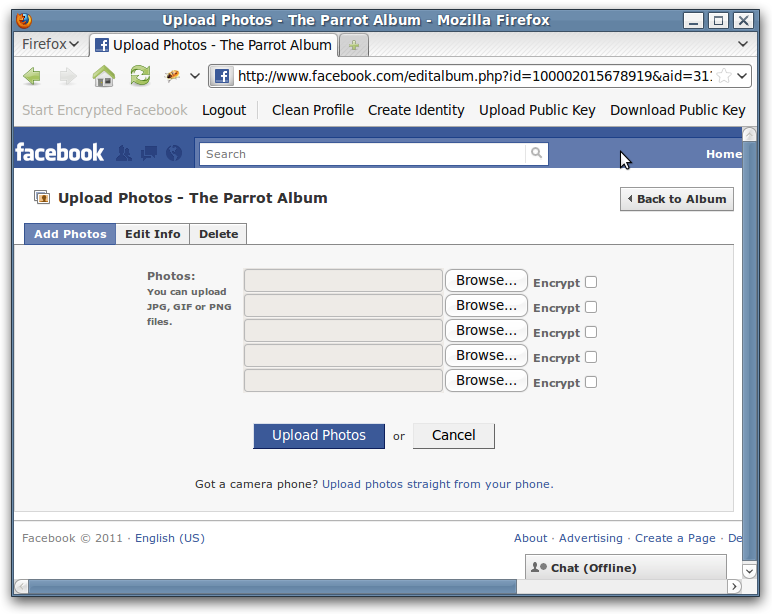
\includegraphics[width=12cm]{screens/pic-upload.png}

            \caption{Input fields and controls for submitting encrypted images.}
            \label{scn:pic-up}
        \end{center}
    \end{figure}


\subsection{Posting a comment}
A user has navigated to his news feed. He wishes to write an encrypted reply to a plaintext comment on a news feed post of an encrypted photo. It is assumed he already possesses the public keys required and can decrypt the photo in question.

\begin{desc}

    \item[Action Sequence] \hfill
    \begin{enumerate}
        \item Select the comment box below the plaintext reply.
        \item Type comment in plaintext.
        \item Click the {\tt [Encrypt \& Submit]} button.
        \item Use the friend selector to select recipients and submit.
        \item Refresh the page to review comment.
    \end{enumerate}
    
    \item[Defence of Credibility] \hfill
        \begin{itemize}
            
            \item User knows to select the comment box. This is required for submitting a plaintext comment, we assume the user will try the method they are used to.
            
            \item User knows things are OK as the {\tt [Encrypt \& Submit]} appears once the textbox has focus.
            
            \item User knows to type in the comment - this is identical to submitting a plaintext comment.
            
            \item User knows to click {\tt [Encrypt \& Submit]}. The user is familiar with clicking a similar submit button during plaintext entry. The button is positioned beside the {\tt [Submit]} for plaintext entry, is styled like the {\tt [Submit]} button and is clearly labelled. Submitting an encrypted comment is part of the original task.
            
            \item User knows how to use the recipient selector (see Appendix \ref{app:cw:sel}).
            
            \item User knows things are OK as Facebook handles the submission process from here as per normal. A loading icon appears briefly, then the comment itself appears.
            
            \item User knows that their submission was encrypted as this fact is stated as part of the comment encoding.
            
            \item User knows they must refresh the page to view their own comment. Even if this is their first encrypted submission, Facebook users will be familiar with the process of refreshing a page when something is not working or to view an update. If the user does not make the connection right away, they should realise that encrypted text submissions are decrypted as a page first loads when they return to the page and see the item decrypted automatically.
        
        \end{itemize}
\end{desc}


    \begin{figure}[tbph]
        \begin{center}
        
                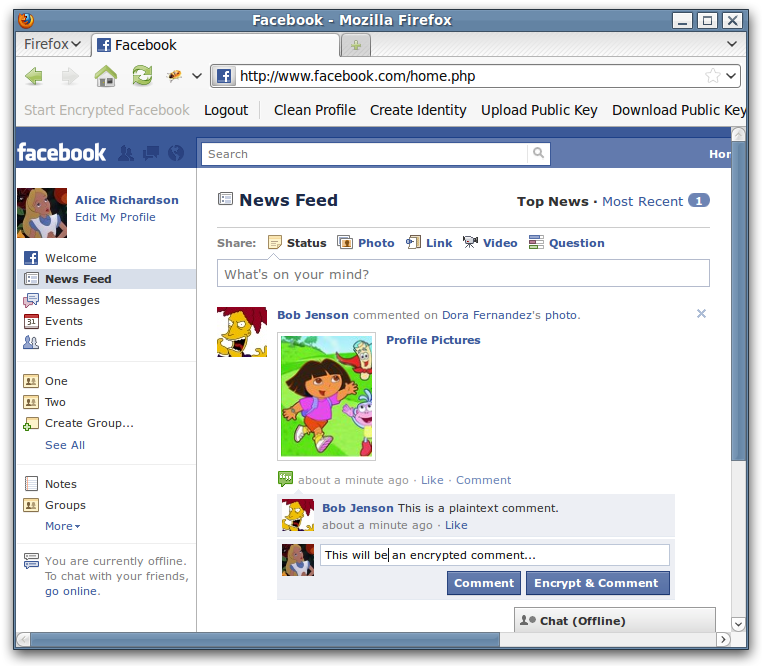
\includegraphics[width=12cm]{screens/comment.png}

            \caption{Input fields and controls for posting a comment to a news feed entry.}
            \label{scn:comment}
        \end{center}
    \end{figure}
\cleardoublepage%*****************************************
\chapter{Conclusion}\label{ch:conclusion}
%*****************************************

\section{Evaluation of Requirements}

It works, and works for groups of 400 - covered by cognitive walkthrough. Also group size of 400 made possible by image method.

Should be unobtrusive - security holes we dealt with according to threat model, best compromise we can come up with. Timing breakdown says not waiting around. Cognitive walkthrogh demonstrates portability.

Incremental deployment - refer to implementation, we nailed this trivially. On a subjective note refer to the steganography also.

Extensible library components - refer to implementation, abstract factory groups families of components. Also refer to image method evaluation - clearly had to swtich between them to run those tests.

\section{Retrospective}

What I would have done differently?

No point in implementing Haar since it has poor poor capacity.

Pushed more stuff in to the C library, then have a very thin JavaScript layer on top. Could use same underlying library for different browsers, with slightly tweaked JS extension for each. Would require using htmlcxx or similair, so no easy JavaScript DOM walking - but tradeoff is that no messing around going back and fourth between two languages, instead just writing a C++ aplication and a wrapper for it.

Tighter integration between FEC and conduit image - combine the two. Was never any real need to separate them.

Added multithreading just because there is probably plenty of opportunity for parallelism.

Add backwards compatibility of difference versions as a requirement; store the encoding method in each image when encoding; allow choosing the decoding method on the spot at decode time rather than at initialisation. Since user base is very important (network effects etc.) and so splitting the user base in any way is very bad.

\section{Future work}

Would be great if we could use ECC encryption because overhead would be cut by a big factor, though patent issues etc. mean bad.

Would be great to find an optimal solution to the image problem. Practically it doesnt make much difference but from a theoretical perspective its interesting - could easily turn into a thesis.


\section{Potential deployment}

Obviously would need to expand threat model and deal with security holes. Also need to relax certain constraints i.e. more character support for languages other than English.

Main problem is Linux-only at the moment. Wouldn't take too much trouble to compile on Windows though. (as if).

The idea about seperating headers from content is cool. Would be nice to experiment regarding the performance hit, but essentially we could have sliding parameter which indicated security vs storage overhead tradeoff.




% *******************************************************************
%   Appendix and bibliography
%********************************************************************
\addcontentsline{toc}{chapter}{Bibliography}
\cleardoublepage\printbibliography
\cleardoublepage\part*{Appendix}
\appendix
\cleardoublepage\chapter{Codec Timing}

Figure \ref{graph:codec-speeds} shows a comparison of encode and decode times across varying quality factors for each of the conduit image implementations. Due to limited testing equipment and the length of the tests CPU load could not be kept uniform - these results give only an approximation of the timing involved. Section XXX gives a more accurate overview of time spent encoding and decoding for the 3-bit scaling conduit image class.

\begin{figure}[tbph]
  \begin{center}
    
\subfigure{
\begin{tikzpicture}
    \begin{axis}[grid=major,xlabel=JPEG Quality Factor,ylabel=Encoding time (ms),
    height=5cm,width=10cm,legend style={legend pos=outer north east}]
    
    \addplot
        table[x=QF,y=e_Sc3] {gfx/encoding_time.data};
    
    \addplot
        table[x=QF,y=e_Sc4] {gfx/encoding_time.data};
        
    \addplot
        table[x=QF,y=e_Haar] {gfx/encoding_time.data};
        
    \legend{Scaled3,Scaled4,Haar}
    
    \end{axis}
\end{tikzpicture}
}
\subfigure{
\begin{tikzpicture}
    \begin{axis}[grid=major,xlabel=JPEG Quality Factor,ylabel=Decoding time (ms),
    height=5cm,width=10cm,legend style={legend pos=outer north east}]
    
    \addplot
        table[x=QF,y=d_Sc3] {gfx/encoding_time.data};
    
    \addplot
        table[x=QF,y=d_Sc4] {gfx/encoding_time.data};
        
    \addplot
        table[x=QF,y=d_Haar] {gfx/encoding_time.data};
        
    \legend{Scaled3,Scaled4,Haar}
    
    \end{axis}
\end{tikzpicture}
}

    \caption{Per image encode and decode times for each of the three conduit image implementations, for varying JPEG quality factors.}
    \label{graph:codec-speeds}
  \end{center}
\end{figure}

\begin{figure}[tbph]
    \begin{center}
\begin{tikzpicture}
\begin{axis}[xlabel=Time (seconds), ylabel=Frequency,
grid=major,const plot, ymin=0, enlargelimits=false,
width=12cm, height=5cm, legend style={area legend}]

    \addplot[fill=blue, fill opacity=0.5] table[x=t,y=Text] {gfx/async_text_hist.data};
    
    \addplot[fill=red, fill opacity=0.5] table[x=t,y=Text_c] {gfx/async_text_hist.data};
    
    \addplot+[sharp plot,blue, mark=no marker] coordinates
        {(6.403,0) (6.403,56)};
        
    \addplot+[sharp plot,red, mark=no marker] coordinates
        {(3.463,0) (3.463,56)};
    
    \legend{Cache off,Cache on}
\end{axis}
\end{tikzpicture}

\begin{tikzpicture}
\begin{axis}[xlabel=Time (seconds), ylabel=Frequency,
grid=major,const plot, ymin=0, enlargelimits=false,
width=12cm, height=5cm, legend style={area legend}]
    
    \addplot[fill=blue, fill opacity=0.5] table[x=t,y=Images] {gfx/async_image_hist.data};
    
    \addplot[fill=red, fill opacity=0.5] table[x=t,y=Images_c] {gfx/async_image_hist.data};
    
    \addplot+[sharp plot,blue, mark=no marker] coordinates
        {(19.169,0) (19.169,130)};

    \addplot+[sharp plot,red, mark=no marker] coordinates
        {(4.067,0) (4.067,130)};
    
    \legend{Cache off,Cache on}
    
\end{axis}
\end{tikzpicture}
    \caption{Histogram of 400 page loading times for newsfeeds containing 15 encrypted messages (top) and 15 encrypted images (bottom).}
    \label{graph:hist}
  \end{center}
\end{figure}


\begin{figure}[tbph]
    \begin{center}
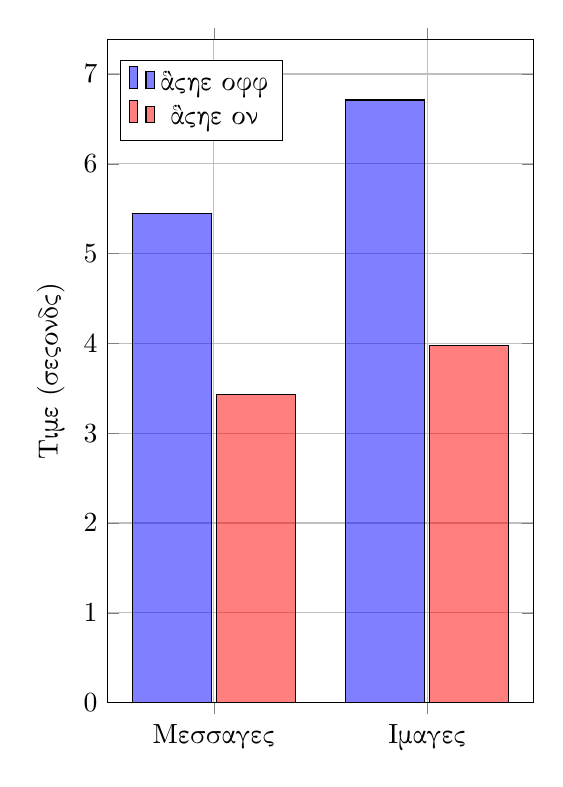
\begin{tikzpicture}
\begin{axis}[grid=major,ybar, 
    symbolic x coords={Messages,Images},
    xtick=data,ylabel=Time (seconds), width=7cm, height=10cm,
    legend style={legend pos=north west, area legend},
    bar width=1cm,enlarge x limits=0.5,ymin=0]
        \addplot[fill=blue, fill opacity=0.5] coordinates { (Messages,5.4457) (Images,6.7105) };
        \addplot[fill=red, fill opacity=0.5] coordinates { (Messages,3.4306) (Images,3.9765) };
        \legend{Cache off, Cache on}
\end{axis}
\end{tikzpicture}
    \caption{Average time before first encrypted item loads.}
    \label{graph:time-first}
  \end{center}
\end{figure}

\begin{figure}
    \begin{center}
        \begin{tikzpicture}
        \begin{axis}[grid=major,ycomb,
        ylabel=Time (ms), 
        width=12cm, height=5cm,
        bar width=0.3cm, ymin=0, xmin=2, xmax=15, enlarge x limits=0.04]
            \addplot[blue] table[x=Item,y=Text] {gfx/async.data};
        \end{axis}
        \end{tikzpicture}
        \begin{tikzpicture}
        \begin{axis}[grid=major,ycomb,
        ylabel=Time (ms), xlabel=Message,
        width=12cm, height=5cm,
        bar width=0.3cm, ymin=0, xmin=2, xmax=15, enlarge x limits=0.04]
            \addplot[red] table[x=Item,y=Text_c] {gfx/async.data};
        \end{axis}
        \end{tikzpicture}
    \caption{Average time interval between successive message loads, with caching turned off and on (top and bottom respectively).}
    \label{graph:txt-rest}
    \end{center}
\end{figure}

\begin{figure}[tbph]
\begin{center}
    
\begin{tikzpicture}
\begin{axis}[grid=major,ycomb,
ylabel=Time (ms), 
width=12cm, height=5cm,
bar width=0.3cm, ymin=0, xmin=2, xmax=15, enlarge x limits=0.04]
    \addplot[blue] table[x=Item,y=Image] {gfx/async.data};
\end{axis}
\end{tikzpicture}

\begin{tikzpicture}
\begin{axis}[grid=major,ycomb,
ylabel=Time (ms),xlabel=Image,
width=12cm, height=5cm,
bar width=0.3cm, ymin=0, xmin=2, xmax=15, enlarge x limits=0.04]
    \addplot[red,] table[x=Item,y=Image_c] {gfx/async.data};
\end{axis}
\end{tikzpicture}

\caption{Average time interval between successive image loads, with caching turned off and on (top and bottom respectively).}
\label{graph:img-rest}
\end{center}
\end{figure}
\cleardoublepage\chapter{Project Proposal}

\section*{Introduction and Description of the Work}

Facebook is a social networking service that, as of July 2010, has over 500 million users worldwide. Many people have recently become increasingly worried about Facebook's rather relaxed attitude towards the privacy of personal data. However, attempts at building more secure social networks with technical solutions that ensure data privacy, such as encryption, have not enjoyed much success because Facebook capitalises on the network effect of everyone else using it.

It would be very useful if we could still use Facebook, but encrypt all the data stored there, enabling only those who use the same tool (and possess the appropriate key) to see the plaintext. Obvious targets for encryption are profile information, pictures and comments or other public messages exchanged between users. Extensions might include encrypting videos, events and other information. Ideally, the system would be as unobtrusive as possible; encryption/decryption options should be integrated as if they were implemented by Facebook itself.

Several possible approaches exist for this project. One approach would be to develop a standalone extension for the Firefox web browser (or possibly some other extensible browser such as Chrome). A second would be to develop a 'userscript' for Greasemonkey, an existing Firefox extension. This approach would afford some cross browser compatibility since userscripts are gaining limited support on browsers other than Firefox. Both these approaches would be a form of augmented browsing, relying on modifying web pages on the fly just before they are displayed.

A further (and potentially much more complicated) method would be to develop a complete client. This could be either a web-based or desktop client. In either case, creating a fully functional Facebook site clone would likely be beyond the scope of this project - however developing a cut down version should at least be considered. The project's first goal would be to assess the suitability of each of these approaches.



\section*{Starting Point}

Existing experience writing web pages with HTML and CSS. Awareness of JavaScript and tools such as Greasemonkey. Some aspects from the Security courses in Part IB and Part II Computer Science will likely be required.


\section*{Substance and Structure of the Project}


The project can be broken down into the following main sections. We assume here that the implementation takes the form of the plugin, though as mentioned previously this may not ultimately be the case.

\begin{enumerate}

\item Research each of the possible methods of implementation. Choose the most suitable approach.

\item Implement a method of submitting encrypted data to Facebook. Any encrypted data needs to be recognisable as such, e.g. via some kind of tag. Targets for encryption would be photographs, comments and profile information.

\item Implement a method of recovering and displaying encrypted data.

\item Implement a method of key exchange and storage between extension users.

\item Modify the Facebook user interface so that recovery and display of encrypted data happens seamlessly. Ensure an appropriate response for encrypted data for which the user does not have a key.

\item Modify the Facebook user interface so that encrypted submission and key exchange can be done seamlessly by the plugin user.

\item Extend the plugin to improve interaction with users who do not have the plugin installed. Allow the creation of appropriate default behaviors for communicating with users who do/do not themselves have the plugin (which conversations should be encrypted and which shouldn't). Recognizing certain actions and prompting the user may be necessary. Another example - making tags marking content as encrypted more human readable, rather than just perceived gibberish.

\item Demonstrate the plugin by creating a sample set of profiles and performing a set of test actions successfully. Document and record the results.

\item Record various loading times and analyse the performance of the extension.

\item Perform a cursory analysis of the plugins theoretical running time on various actions, with regard to input length and number of users. Demonstrate (as much as possible) that the plugin would be viable for large scale adoption, taking into account the number of Facebook users worldwide.

\item As a possible extension, implement more extensive user interface alterations to change the aesthetic of the encrypted Facebook user experience (e.g. different colour schemes, more tightly integrated, inline icons/controls). This would increase ease of use and make it more immediately clear to any user whether or not they have the plugin enabled.

\item As a possible extension, implement and/or demonstrate compatibility across a range of platforms. Several browsers (other than Firefox) have limited support for userscripts, for example. If writing a standalone plugin, this could perhaps be ported to other browsers (e.g. Chrome, Opera) or operating systems (e.g. Android, iOS).

\item As a possible extension, create a complementary Facebook Application that allows combining encryption options with Facebook's existing privacy controls (among other possible improvements).

\item As a possible extension, extend encryption beyond just comments, photos and profile information. Possibly interesting features might be completely encrypted profile creation (including full name); encrypted events and attendees; encrypted 'pages' and 'likes'; encrypted dates and locations.

\item As a possible extension, look at incorporating steganography techniques (hiding encrypted data in pictures or videos, for example). This might not only clean up the user experience for non-extension users, but preempt any preventative measures Facebook might take to block use of the plugin.

\item Repeat any analysis (particularly of performance) for any completed extensions, as required.


\end{enumerate}


\section*{Resources Required}

None.


\section*{Success Criterion}

For the project's core functionalities, each of the following requirements should be met. For any completed extensions, discussion should at least be made on whether the requirements are met, can/could be met with further development, or otherwise.

\begin{enumerate}

\item The plugin should be able to perform the set of initial test actions on a set of purposely created test profiles, demonstrable by annotated screenshots. The test actions should provide evidence of successful submission and recovery of photos, comments and profile information, as well as key exchange.

\item The encryption scheme used should ensure at least confidentiality of data and should be immune to any brute force decryption attack.

\item Assuming the previous requirement is met; under analysis, the plugin should perform within acceptable limits for the majority (greater than 95\%) of target users in regard to page loading times. A reasonable definition of acceptable limits should be used (e.g. http://www.useit.com/papers/responsetime.html). Target users are defined as those capable of installing the plugin, thus accurate statistics on typical connection speeds for Facebook users (not including those on mobile devices who would not be able to use the plugin in any case) should be investigated.

\item Analysis of the plugin's operation should demonstrate, superficially at least, that the schemes used would scale up if adoption took place among groups of users larger than the small number of test profiles. If required, define large scale adoption as use among at least 1\% of worldwide Facebook users. This will likely require some research into Facebook limitations on, for example, the length of text inputs.


\end{enumerate}







\section*{Timetable and Milestones}

\subsection*{October 25th - November 1st}

Complete a skeleton project with all required sections. Set up version control and review any other library/programming requirements that need to be considered before coding can begin.

If required, begin the process of setting up a certification authority service. Make an initial indication of what schemes will be used for encryption/decryption, key exchange and authentication

Create a prototype Greasemonkey userscript that interacts somewhat with Facebook. Test Greasemonkey's limits, particularly on storing data persistently when browsing from page to page and fetching/parsing additional pages. Repeat this process with a simple Firefox (or alternative browser) extension. At this point it should become clear which approach (userscript, extension or full client) will be most suitable.

Milestones: Project skeleton complete. Two working test applications (Greasemonkey and standalone plugin) that demonstrate simple interaction with Facebook.


\subsection*{November 1st - November 15th}

Many possible extensions have been stated for this project - here initial research into their feasibility should be performed.

By the end of this period, a prototype implementation which can encrypt and decrypt text fields (i.e. comments and profile information) will be complete. At this point the user will need to manually select fields for encryption/decryption and supply the appropriate key.

Milestone: First working prototype in place.

\subsection*{November 15th - December 3rd (end of Michaelmas term)}

Encryption should be extended to images as well as text fields.

Some automation added to the recovery process. The system should now parse the page and work out what elements may be decrypted. The user will still have to supply the appropriate keys manually.

Milestone: Second working prototype completed, as described.


\subsection*{December 4th (Winter vacation starts) - December 25th}

The prototype should now be extended to manage keys automatically. If a CA service exists/is needed then the software should interface with it appropriately. Key exchange hasn't yet been integrated into the browser however.

Recovery of elements can now be done in complete autonomy - we can parse what needs to be recovered, work out what can be recovered, then do so. Again, at this stage, no changes have been made to the Facebook web interface.

Work should begin on the first two written sections of the Dissertation (Introduction and Preparation).

Milestone: Third prototype with working authentication and secure key exchange.

\subsection*{December 26th  - January 17th (Winter vacation ends)}

During this period modifications should now be made to the Facebook UI to integrate actions into the web page itself. Modification do not need to be attractive (that is left for a later possible extension) but all possible actions should now be able to be initiated through the Facebook site

By the end of the vacation there should exist a draft of the Introduction section and the contents of the Preparation section should be mapped out.

Milestone: Fourth prototype with all core functionality complete.

\subsection*{January 18th (Lent term begins) - January 25th}

Polishing of the final application should be made. Informal testing and any necessary tweaks/optimizations should be completed. Useability improvements implemented, e.g. settings and configurations options should be added for default behaviors. Tags should be re-done in a more human readable form.

Introduction and Preparation sections should be complete and work should be underway on the Implementation section.

\subsection*{January 26th - February 18th }

During this period, any extensions should be implemented. The Implementation chapter should be nearing completion, bar any extension work which needs writing up.

The progress report presentations fall during this period; clearly if the project is on track then there will be plenty to talk about. Since implementation should be nearing completion this is also a good point for a project review.

Milestones: All programming and implementation completed, leaving only testing, analysis and writing up left to complete. Progress Report Deadline - Fri 4 Feb 2011. Entire project reviewed both personally and with Overseers.


\subsection*{February 18th - March 11th}

Complete any outstanding implementation work on possible extensions. Perform testing and obtain all results to be used in the analysis of the project. Ideally all testing should be complete, though again possible extension work may leave a small amount left to be done.

Milestones: Complete draft of the first three chapters (Introduction, Preparation and Implementation). Testing and analysis completed.

\subsection*{March 11th - March 18th (end of Lent term)}

During this week the final two chapters (Evaluation and Conclusion) should be written up, completing a full draft of the dissertation.

Milestones: First complete draft of dissertation.

\subsection*{March 19th (start of Easter vacation) - March 26th }

Review the entire dissertation. Insert any diagrams, graphs, tables and references which remain outstanding. Tweak advanced project presentation details such as formatting of code snippets. Focus on concision; remove any perceived wordiness and ensure project word count lies within the required range.

Milestones: Second complete draft, now ready for submission to DoS/supervisor.

\subsection*{March 27th - April 25th (end of Easter vacation)}

During this 4 week period much time will be taken up by exam revision.

Submit the project to supervisors, DoS, fellow students and parents. Any feedback should be taken into account and the dissertation revised where necessary.

Milestones: By the end of the vacation have project complete and ready to submit.


\subsection*{April 25th - May 20th}

This time should be left exclusively for exam revision. There should however, be just enough time to re-read the dissertation and make any final alterations, before final submission one week before the deadline.

Milestones: Submission of Dissertation - Friday 20th May. Date one week prior to deadline - Friday 13th May.



%********************************************************************
%   Other Stuff in the Back
%********************************************************************


%********************************************************************
%   End of document
%********************************************************************
\end{document}
